\documentclass[12pt, а4paper]{article}
\usepackage[T1, T2A]{fontenc}
\usepackage[utf8]{inputenc}
\usepackage[serbianc]{babel}
\usepackage[margin=1in]{geometry}
\usepackage{graphicx}
\usepackage{tocloft}
\usepackage[unicode, breaklinks]{hyperref}

%\usepackage{hyperref}
%\PassOptionsToPackage{hyphens}{url}\usepackage{hyperref}

\usepackage{caption}
%%%%%%%%%%%%%%%%%%%%%%%%%%%
\usepackage{amsmath}
\usepackage{mathtools}
\DeclarePairedDelimiter\ceil{\lceil}{\rceil}
\DeclarePairedDelimiter\floor{\lfloor}{\rfloor}
%%%%%%%%%%%%%%%%%%%%%%%%%%%
\usepackage{float}
\usepackage{minted}
\usepackage{verbatim}
\usepackage{cite}
\usepackage[nottoc]{tocbibind}
\usepackage{romannum}

%\usepackage[none]{hyphenat}
\tolerance=1
\emergencystretch=\maxdimen
\hyphenpenalty=10000
\hbadness=10000

\bibliographystyle{ieeetr}
%\setlength{\bibsep}{0.0pt}

\hypersetup{
    colorlinks=true,
    linkcolor=black,
    citecolor=black,
    filecolor=magenta,      
    urlcolor=cyan,
}
\makeatletter
\g@addto@macro\UrlBreaks{\do\-}
%\g@addto@macro{\UrlBreaks}{\UrlOrds}
\makeatother

%\hyphenpenalty 10000

\newcommand{\CS}{C\nolinebreak\hspace{-.05em}\raisebox{.6ex}{\tiny\bf \#}}

\usepackage{enumitem}


\begin{document}
%\sloppy
\pagenumbering{gobble}

\begin{titlepage}
%\newgeometry{margin=1in}
%\fontsize{14}{×}
\center
\Large
Универзитет у Крагујевцу\\
Факултет инжењерских наука\\
\vspace{0.8cm}

\includegraphics[scale=0.5]{slike/grb}\\
\vspace{0.8cm}
Дипломски рад\\
Програмирање система који раде у реалном времену\\
\vspace{1.7cm}
\Huge
\textbf{Детекција карата за игру коришћењем YOLO алгоритма за детекцију објеката}\\
%\vspace{5cm}
\vfill
\large
\flushleft Студент: \hfill Професор:\\
\vspace{0.1cm}
Алекса Величковић 576/2015\hfill др Владимир Миловановић\\
%\vspace{0.1cm}
%Алекса Величковић 576/2015\\
%\vfill
\vspace{1.3cm}
\center
Крагујевац, септембар 2020.\\
%\restoregeometry
\end{titlepage}

\tableofcontents
\newpage

\pagenumbering{arabic}
\section{Увод}
У овом раду ће бити описана реализација система за детекцију карата за игру.
Биће објашњена припрема слика над којима се тренира вештачка неуронска мрежа, 
начин рада YOLO алгоритма,
поступак тренирања вештачке неуронске мреже и начин покретања система.

Свака карта је снимљена под различитим осветљењем у кратком видеу из кога се добијају слике;
дефинисана је позиција знака и броја карте, па се насумичним позиционирањем карте преко
насумично изабране позадине генерише скуп слика над којима се врши тренирање.

Тренирање над сликама је извршено коришћењем Darknet
програмског оквира за вештачке неуронске мреже и омогућава детекцију над сликом,
видеом и у реалном времену са камере.

Пројекат се може посматрати као први корак у прављењу
карташке игре која је под контролом рачунара. Рачунар би
коришћењем овог система детектовао карте, а у другом кораку би,
при свакој детекцији, одредио који играч је ту карту одиграо.
Игра би укључивала четири играча и сваки би био придружен
страници слике са камере. \mbox{По детектовању карте}, одредило би се
са које стране је ушла рука играча у кадар и њему би била додељена
детектована карта.

YOLO алгоритам је могуће применити за детекцију било којих
објеката и овим пројектом се показује „пут” од снимка објекта
до програма који га детектује у потпуно другачијим условима и
у стању је да то уради невероватно брзо,
чак у реалном времену.


\newpage
\section{Припрема тренинг скупа}
Генерисање слика за тренирање је реализовано коришћењем
Jupyter свеске \verb creating_playing_cards_dataset.ipynb ,
која се налази у GitHub репозиторијуму, наведеном у литератури \cite{git_karte}.
\subsection{Добијање слика из видеа}
Свака карта је снимљена приближно 20 секунди под различитим осветљењем.
Из сваког снимка је потребно издвојити само карту и сачувати све слике као \textit{.png} датотеке.
Програм генрише око 100 слика карата по видеу.

Прво, потребно је направити шаблон тј.\ правоугаоник, који ће имати однос дужинa страница исти као и карта
коришћеног шпила. Пошто су у првој „ћелији” (сегменту кода) Jupyter свеске дефинисане дужина
и ширина (mm) карте одговарајућег шпила,
линијама кода \verb cardW=56  и \verb cardH=86  (слика \ref{fig:karta_dim}),
тако се следећим кодом прави шаблон (маска):
\begin{minted}{python}
bord_size=2 # bord_size alpha=0
alphamask=np.ones((cardH,cardW),dtype=np.uint8)*255
cv2.rectangle(alphamask,(0,0),(cardW-1,cardH-1),0,bord_size)
cv2.line(alphamask,(bord_size*3,0),(0,bord_size*3),0,bord_size)
cv2.line(alphamask,(cardW-bord_size*3,0),(cardW,bord_size*3),0,bord_size)
cv2.line(alphamask,(0,cardH-bord_size*3),(bord_size*3,cardH),0,bord_size)
cv2.line(alphamask,(cardW-bord_size*3,cardH),
				   (cardW,cardH-bord_size*3),0,bord_size)
plt.figure(figsize=(10,10))
plt.imshow(alphamask)
\end{minted}

Неопходно је да карта буде јасно издвојена од позадине, узимајући у обзир и ћошкове који су закривљени;
па се после стварања правоугаоника, позивом функције \verb cv2.rectangle() , црта и сваки од ћошкова
функцијом \verb cv2.line() .

\newpage
Извршавањем дела кода, наведеног изнад, се приказује описани правоугаоник, као на слици \ref{fig:maska}.

\begin{figure}[H]
  \centering
      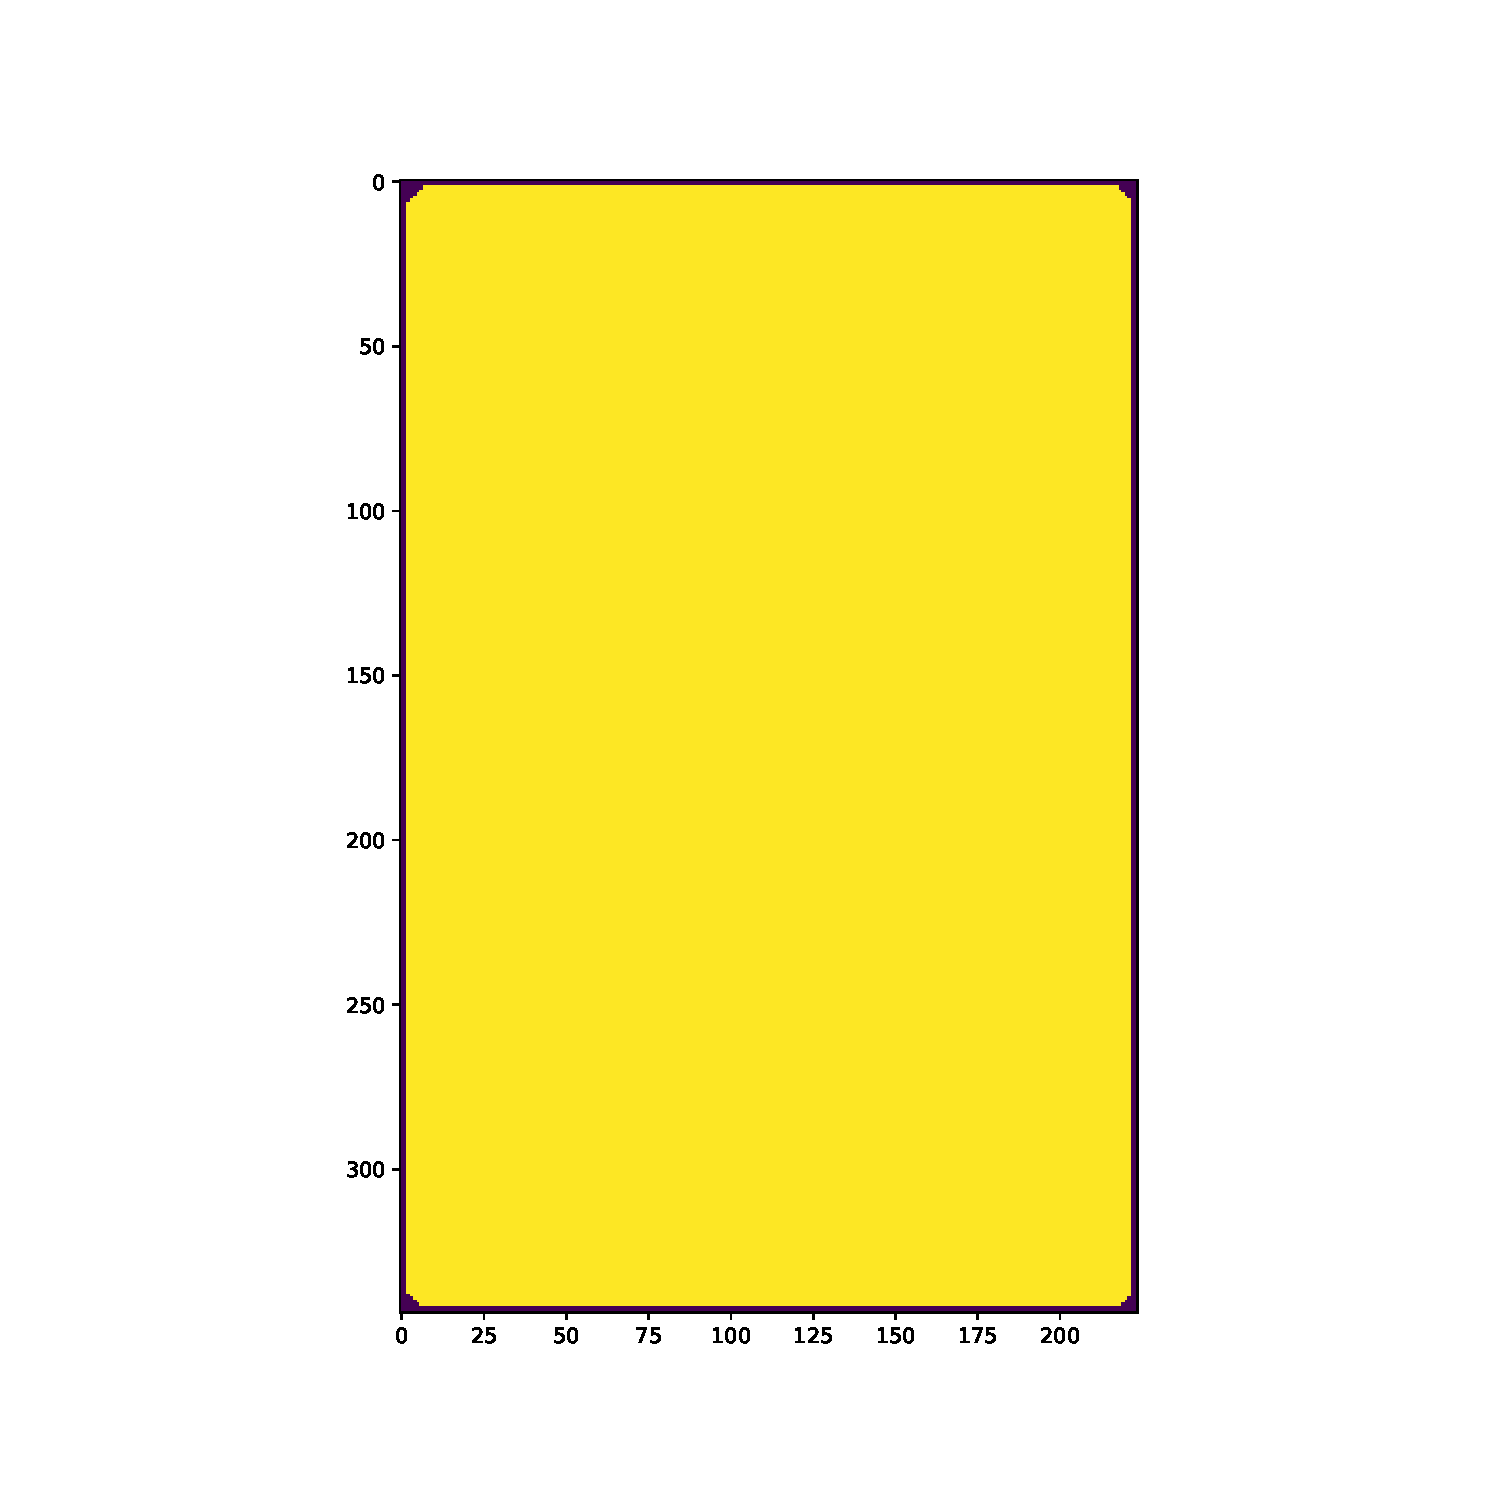
\includegraphics[scale=0.4]{slike/alphamask.pdf}
  \caption{Шаблон за издвајање карте са снимка}
  \label{fig:maska}
\end{figure}

Сада се дефинише функција \verb extract_card() , која издваја карту из прослеђене слике.
На њеном почетку се врши провера замућења слике позивом функције \verb varianceOfLaplacian() , која
враћа варијансу Лапласове функције позивом \verb cv2.Laplacian(img,cv2.CV_64F).var() . Јасна слика
би требало да има високу варијансу \cite{stack_slika}. У наредном кораку се слика претвара у
црно-белу са и над њом позива неколико филтера. Позивом \verb cv2.bilateralFilter()  се смањује шум
на слици и овај филтер не утиче на ивице (прелазе) на слици; након тога се издвајају ивице са слике
позивом \verb cv2.Canny() . После извршених филтрирања, потребно је наћи контуре
на слици коју смо добили
(са наглашеним ивицама) и то се извршава са \verb cv2.findContours() , где контура представља криву
која спаја све тачке дуж границе, исте боје и интензитета \cite{cv2_kontura}. Претпостављено је
да највећа препозната контура представља карту, па се она добија сортирањем свих издвојених контура
у опадајућем редоследу и издвајањем прве из листе. Проверава се да ли је добијена контура
правоугаоног облика, тако што се изврши однос површина контуре и најмањег правоугаоника
који је окружује и уколико су вредности приближне, променљива \verb valid  има вредност \verb True .

Уколико је утврђено да је пронађена контура правоугаоник, желимо да претворимо простор унутар
контуре у правоугаоник димензија карте из коришћеног шпила.



\begin{minted}{python}
def varianceOfLaplacian(img):
    return cv2.Laplacian(img, cv2.CV_64F).var()
\end{minted}
\newpage
\begin{minted}{python}
def extract_card (img, output_fn=None, min_focus=120, debug=False):
    imgwarp=None    
    # Check the image is not too blurry
    focus=varianceOfLaplacian(img)
    if focus < min_focus: 
        if debug: print("Focus too low :", focus)
        return False,None
    
    # Convert in gray color
    gray = cv2.cvtColor(img,cv2.COLOR_BGR2GRAY)
    
    # Noise-reducing and edge-preserving filter
    gray=cv2.bilateralFilter(gray,11,17,17)
    
    # Edge extraction
    edge=cv2.Canny(gray,30,200)
    
    # Find the contours in the edged image
    cnts, _ = cv2.findContours(edge.copy(), cv2.RETR_EXTERNAL, 
			      cv2.CHAIN_APPROX_SIMPLE) #_,cnts, _ = cv2.    
    # We suppose that the contour with largest area corresponds 
				    #to the contour delimiting the card
    cnt = sorted(cnts, key = cv2.contourArea, reverse = True)[0]
    
    # We want to check that 'cnt' is the contour of a rectangular shape
    # First, determine 'box', the minimum area bounding rectangle of 'cnt'
    # Then compare area of 'cnt' and area of 'box'
    # Both areas sould be very close
    rect=cv2.minAreaRect(cnt)
    box=cv2.boxPoints(rect)
    box=np.int0(box)
    areaCnt=cv2.contourArea(cnt)
    areaBox=cv2.contourArea(box)
    valid=areaCnt/areaBox>0.95
    
    if valid:
        # We want transform the zone inside the contour into 
		   #the reference rectangle of dimensions (cardW,cardH)
        ((xr,yr),(wr,hr),thetar)=rect
        # Determine 'Mp' the transformation that transforms 
				  #'box' into the reference rectangle
        if wr>hr:
            Mp=cv2.getPerspectiveTransform(np.float32(box),refCard)
        else:
            Mp=cv2.getPerspectiveTransform(np.float32(box),refCardRot)
        # Determine the warped image by applying
				    #the transformation to the image
        imgwarp=cv2.warpPerspective(img,Mp,(cardW,cardH))
        # Add alpha layer
        imgwarp=cv2.cvtColor(imgwarp,cv2.COLOR_BGR2BGRA)
        
        # Shape of 'cnt' is (n,1,2), type=int with
						#n = number of points
        # We reshape into (1,n,2), type=float32,
				#before feeding to perspectiveTransform
        cnta=cnt.reshape(1,-1,2).astype(np.float32)
        # Apply the transformation 'Mp' to the contour
        cntwarp=cv2.perspectiveTransform(cnta,Mp)
        cntwarp=cntwarp.astype(np.int)
        
        # We build the alpha channel so that we have transparency on the
        # external border of the card
        # First, initialize alpha channel fully transparent
        alphachannel=np.zeros(imgwarp.shape[:2],dtype=np.uint8)
        # Then fill in the contour to make opaque this zone of the card 
        cv2.drawContours(alphachannel,cntwarp,0,255,-1)
        
        # Apply the alphamask onto the alpha channel to clean it
        alphachannel=cv2.bitwise_and(alphachannel,alphamask)
        
        # Add the alphachannel to the warped image
        imgwarp[:,:,3]=alphachannel
        
        # Save the image to file
        if output_fn is not None:
            cv2.imwrite(output_fn,imgwarp)
        
    if debug:
        cv2.imshow("Gray",gray)
        cv2.imshow("Canny",edge)
        edge_bgr=cv2.cvtColor(edge,cv2.COLOR_GRAY2BGR)
        cv2.drawContours(edge_bgr,[box],0,(0,0,255),3)
        cv2.drawContours(edge_bgr,[cnt],0,(0,255,0),-1)
        cv2.imshow("Contour with biggest area",edge_bgr)
        if valid:
            cv2.imshow("Alphachannel",alphachannel)
            cv2.imshow("Extracted card",imgwarp)

    return valid,imgwarp
\end{minted}

Следећи корак је да се издвоје фрејмови из снимка и над њима позива изнад дефинисана функција;
за то је дефинисана функција \verb extract_cards_from_video() .

Поред провера да ли постоје
улазна видео датотека и излазна фасцикла, где ће бити спаковане слике, отвара се
видео датотека коришћењем OpenCV библиотеке са \verb cap=cv2.VideoCapture(video_fn) , а
онда чита фрејм позивом \verb cap.read() . На сваких 5 фрејмова се позива функција \verb extract_card() .
\begin{minted}{python}
def extract_cards_from_video(video_fn, output_dir=None, keep_ratio=5, 
					    min_focus=120, debug=False):
    if not os.path.isfile(video_fn):
        print(f"Video file {video_fn} does not exist !!!")
        return -1,[]
    if output_dir is not None and not os.path.exists(output_dir):
        os.makedirs(output_dir)
        
    cap=cv2.VideoCapture(video_fn)
    
    frame_nb=0
    imgs_list=[]
    while True:
        ret,img=cap.read()
        if not ret: break
        # Work on every 'keep_ratio' frames
        if frame_nb%keep_ratio==0:
            if output_dir is not None:
                output_fn=give_me_filename(output_dir,"png")
            else:
                output_fn=None
            valid,card_img = extract_card(img,output_fn,
				  min_focus=min_focus,debug=debug)
            if debug: 
                k=cv2.waitKey(1)
                if k==27: break
            if valid:
                imgs_list.append(card_img)
        frame_nb+=1
    
    if debug:
        cap.release()
        cv2.destroyAllWindows()
    
    return imgs_list
\end{minted}

Овако дефинисану функцију је потребно позвати над снимцима свих карата и онда
су слике сачуване у фасциклама, посебно за сваку карту.

\subsection{Означавање знака и броја карте на слици}

Поред дефинисања димензија карте коришћеног шпила, на почетку Jupyter свеске
се дефинишу и позиције ћошкова правоугаоника који окружује знак и
број карте, као на слици \ref{fig:karta_dim}, и сачуване су у 
променљивама \verb cornerXmin , \verb cornerXmax ,
\verb cornerYmin  и \verb cornerYmax .

\begin{figure}[H]
  \centering
      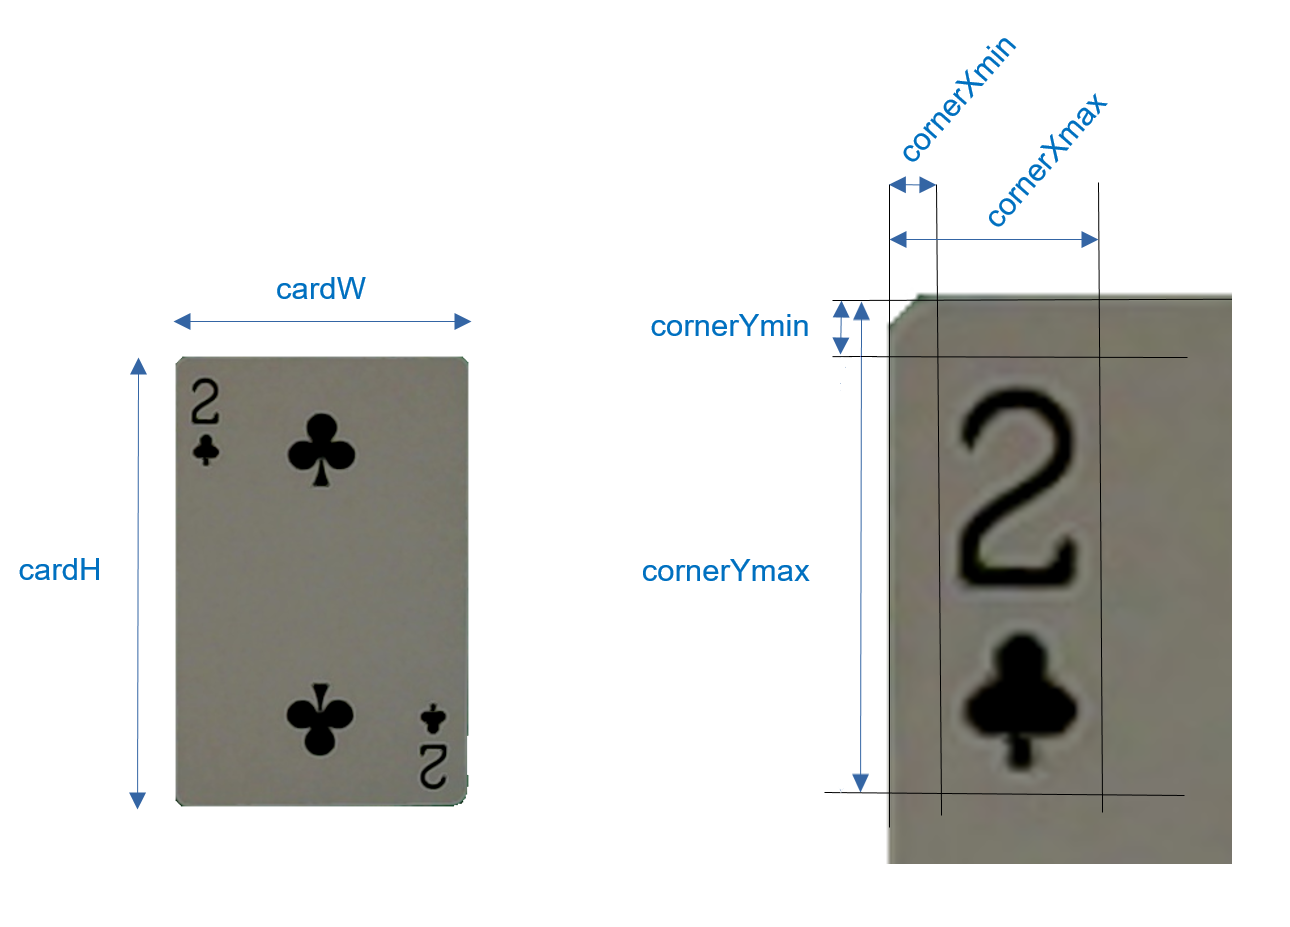
\includegraphics[scale=0.5]{slike/measures.png}
  \caption{Димензије карте и правоугаоника (око броја и знака)}
  \label{fig:karta_dim}
\end{figure}

Потребно је дефинисати функцију која ће унутар овог правоугаоника
одредити контуру унутар које ће се налазити број и знак.

Ова функција је названа \verb find_hull()  и поред слике карте, као
аргумент \verb corner  прима позицију правоугаоника и могуће је проследити
позицију \mbox{горњег-левог} и \mbox{доњег-десног}, а уписани су у променљиве
\verb refCornerHL  и \verb refCornerLR , респективно.

На почетку се издваја део слике означен позицијама правоугаоника и уписује
у променљиву \verb zone . Слика се претвара у \mbox{црно-белу}, издвајају се ивице и
позивом \verb cv2.dilate()  се оне појачавају тј.\ функција ради тако
што промени боју пиксела из црне у белу уколико тај црни
пиксел има испод себе бели \cite{cv2_piksel}. Издвајају се контуре позивом
\verb cv2.findContours()  и дефинишу се минимална површина (\verb min_area )
и минимални однос површина посматране контуре и
конвексног полигона око ње (\verb min_solidity ).

Сада се улази у \verb for  петљу која пролази кроз све нађене контуре;
у њој се прво рачуна површина те контуре, а позивом \verb cv2.convexHull()  се
налази конвексан полигон око контуре.

Функција \verb cv2.moments()  враћа тежиште контуре и потом се 
врше провере:
да ли је површина контуре већа од минимално дефинисане (\verb min_area ),
да ли је однос површина
контуре и конвексног полигона који је окружује већи од минимално дефинисаног
(\verb min_solidity ) и да ли се тежиште контуре налази близу центра
правоугаоника унутар кога је тражена контура.

Све нађене контуре су спојене унутар променљиве \verb concat_contour  и 
сада се одређује коначни полигон око броја и знака, и његова површина. Уколико
је површина полигона у границама минималне и максималне дефинисане вредности
променљива \verb ok  и даље има вредност \verb True , па је још само потребно
позцију полигона дефинисати у односу ивицу карте тј.\ на израчунату позицију,
која је релативна у односу на правоугаоник који је окруживао знак и број,
додати и координате самог правоугаоника у односу на карту.

\begin{minted}{python}
def findHull(img, corner=refCornerHL, debug="no"):
    kernel = np.ones((3,3),np.uint8)
    corner=corner.astype(np.int)

    # We will focus on the zone of 'img' delimited by 'corner'
    x1=int(corner[0][0])
    y1=int(corner[0][1])
    x2=int(corner[2][0])
    y2=int(corner[2][1])
    w=x2-x1
    h=y2-y1
    zone=img[y1:y2,x1:x2].copy()

    strange_cnt=np.zeros_like(zone)
    gray=cv2.cvtColor(zone,cv2.COLOR_BGR2GRAY)
    thld=cv2.Canny(gray,30,200)
    thld = cv2.dilate(thld,kernel,iterations=1)
    if debug!="no": cv2.imshow("thld",thld)
    
    # Find the contours
    contours,_=cv2.findContours(thld.copy(),cv2.RETR_EXTERNAL,
				  cv2.CHAIN_APPROX_SIMPLE) #_,contours,_

    min_area=30 # We will reject contours with small area.
					      #TWEAK, 'zoom' dependant
    min_solidity=0.3 # Reject contours with a low solidity. TWEAK
    concat_contour=None # We will aggregate in 'concat_contour'
				    #the contours that we want to keep    
    ok=True
    for c in contours:
        area=cv2.contourArea(c)
        hull = cv2.convexHull(c)
        hull_area = cv2.contourArea(hull)
        solidity = float(area)/hull_area
        # Determine the center of gravity (cx,cy) of the contour
        M=cv2.moments(c)
        cx=int(M['m10']/M['m00'])
        cy=int(M['m01']/M['m00'])
        #  abs(w/2-cx)<w*0.3 and abs(h/2-cy)<h*0.4 :
        #	TWEAK, the idea here is to keep only the contours
        #		which are closed to the center of the zone
        if area >= min_area and abs(w/2-cx)<w*0.3 and
			abs(h/2-cy)<h*0.4 and solidity>min_solidity:
            if debug != "no" :
                cv2.drawContours(zone,[c],0,(255,0,0),-1)
            if concat_contour is None:
                concat_contour=c
            else:
                concat_contour=np.concatenate((concat_contour,c))
        if debug != "no" and solidity <= min_solidity :
            print("Solidity",solidity)
            cv2.drawContours(strange_cnt,[c],0,255,2)
            cv2.imshow("Strange contours",strange_cnt)
            
     
    if concat_contour is not None:
        # At this point, we suppose that 'concat_contour' contains
        #	only the contours corresponding the value and suit symbols   
        # We can now determine the hull
        hull=cv2.convexHull(concat_contour)
        hull_area=cv2.contourArea(hull)
        # If the area of the hull is to small or too big,
	#	there may be a problem
        min_hull_area=940 # TWEAK, deck and 'zoom' dependant
        max_hull_area=2120 # TWEAK, deck and 'zoom' dependant
        if hull_area < min_hull_area or hull_area > max_hull_area: 
            ok=False
            if debug!="no":
                print("Hull area=",hull_area,"too large or too small")
        # So far, the coordinates of the hull are relative to 'zone'
        # We need the coordinates relative to the image -> 'hull_in_img' 
        hull_in_img=hull+corner[0]
    else:
        ok=False        
    if debug != "no" :
        if concat_contour is not None:
            cv2.drawContours(zone,[hull],0,(0,255,0),1)
            cv2.drawContours(img,[hull_in_img],0,(0,255,0),1)
        cv2.imshow("Zone",zone)
        cv2.imshow("Image",img)
        if ok and debug!="pause_always":
            key=cv2.waitKey(1)
        else:
            key=cv2.waitKey(0)
        if key==27:
            return None
    if ok == False:        
        return None    
    return hull_in_img
\end{minted}

Позивањем функције \verb find_hull()  два пута, једном за \mbox{горњи-леви},
а други пут за \mbox{доњи-десни} правоугаоник, добијају се два полигона, као
на слици \ref{fig:karta_hull}. Ово је потребно извршити над свим картама и
сачувати полигоне у Python речнику, где је кључ назив карте, а његова вредност
је листа која садржи слику карте и позиције два полигона.

\begin{figure}[H]
  \centering
      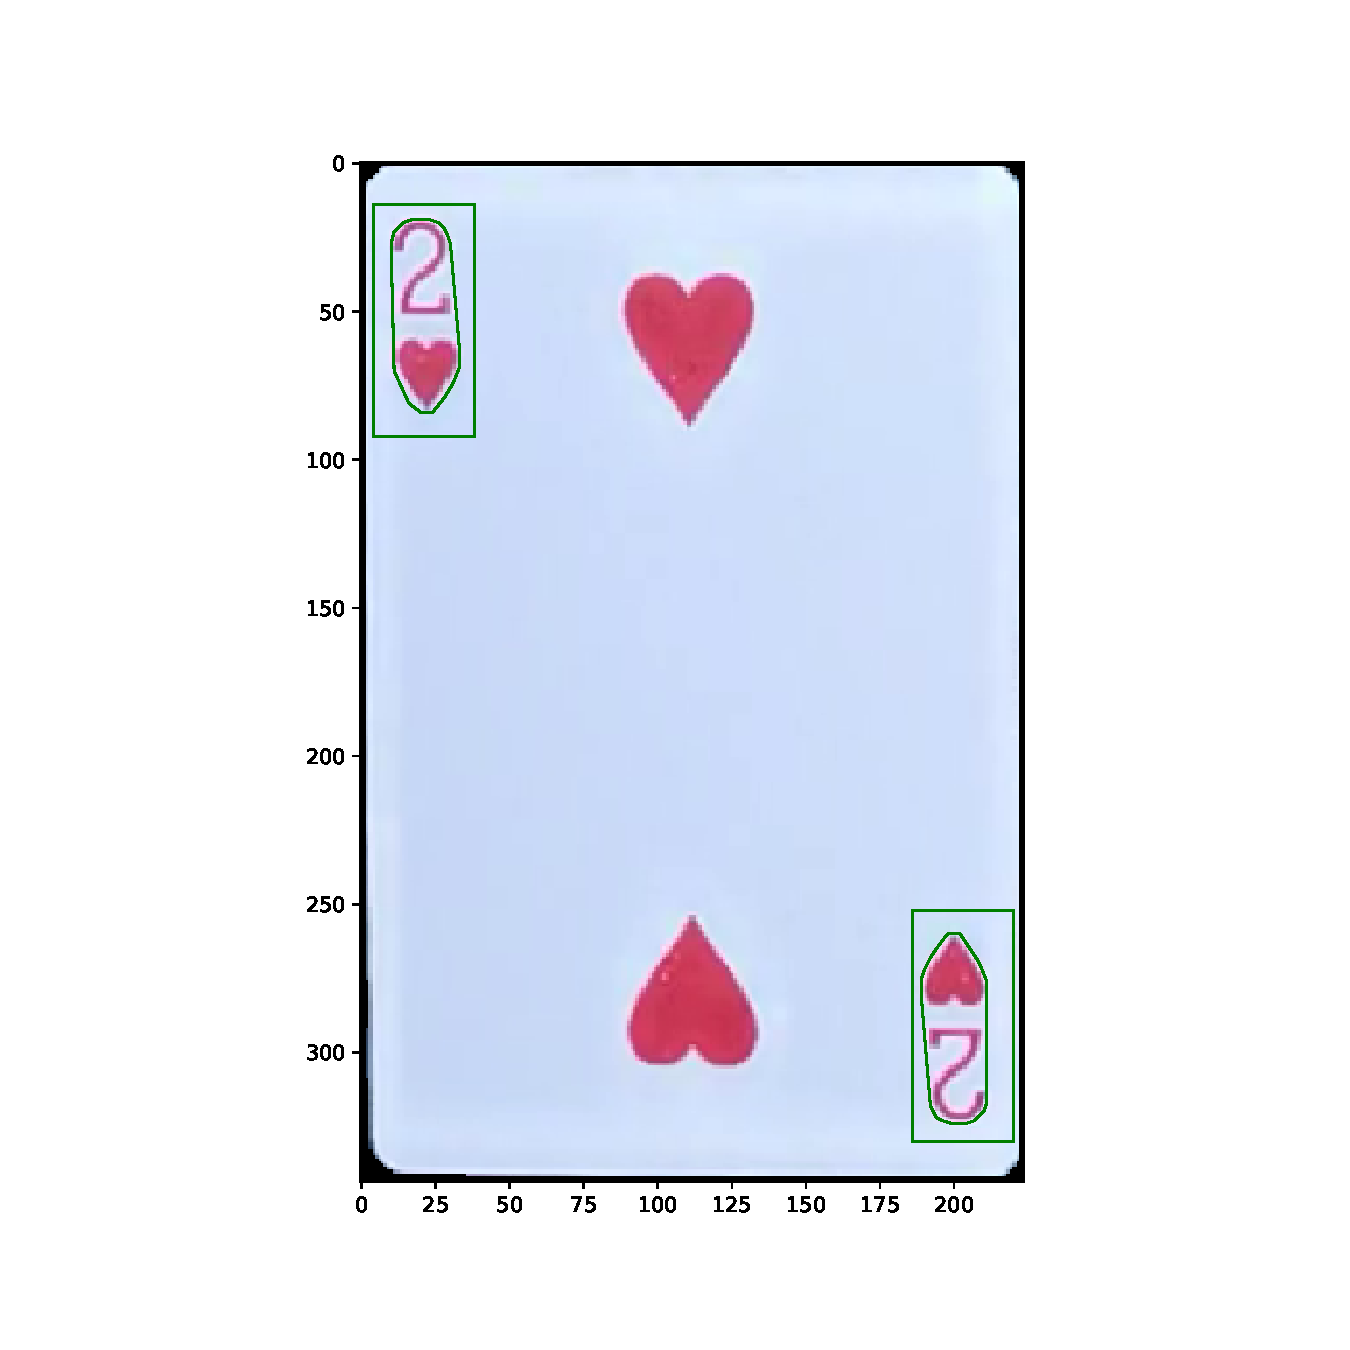
\includegraphics[scale=0.5]{slike/kartaHull.pdf}
  \caption{Полигон који окружује знак и број}
  \label{fig:karta_hull}
\end{figure}

Речник карата \verb cards , са дефинисаним полигонима око знака и броја, се уписује у 
датотеку \verb cards_pck_fn.pck , позивом \verb pickle.dump(cards,open(cards_pck_fn,'wb')) ,
где је коришћен Pickle модул који служи за претварање
Python објеката у ток бајтова и обрнуто \cite{py_pickle}.

\subsection{Прављење скупа за тренирање}

Скуп за тренирање се генерише подвлачењем једне од много позадина испод карата,
а оне се распоређују на два начина:
насумичним транслирањем, ротацијом и увећавањем
две карте; насумичним позиционирањем три карте,
али тако да се налазе једна до друге као када се држе у руци.

Дефинисана је класа \verb Scene , при чијем се инстанцирању у конструктору
позива функција \verb create2CardsScene()  или \verb create3CardsScene() ,
зависно од тога да ли су, као аргументи функције, прослеђене слике две или три карте.
Као аргумент, конструктор прима и слику позадине, поред слика карата и полигона који
окружују њихов знак и број.

Функцијом \verb create2CardsScene()  се извршава распоређивање две карте.
На њеном почетку се позива функција \verb hull_to_kps() , за сваки полигон који
окружује знак и број тј.\ њих четири. 

\begin{minted}{python}
def create2CardsScene(self,bg,img1, class1, hulla1,hullb1,img2,
						class2,hulla2,hullb2):
        kpsa1=hull_to_kps(hulla1)
        kpsb1=hull_to_kps(hullb1)
        kpsa2=hull_to_kps(hulla2)
        kpsb2=hull_to_kps(hullb2)        
        # Randomly transform 1st card
        self.img1=np.zeros((imgH,imgW,4),dtype=np.uint8)
        self.img1[decalY:decalY+cardH,decalX:decalX+cardW,:]=img1
        self.img1,self.lkps1,self.bbs1=augment(self.img1,
				[cardKP,kpsa1,kpsb1],transform_1card)
        # Randomly transform 2nd card. We want that card 2
        #		does not partially cover a corner of 1 card.
        # If so, we apply a new random transform to card 2
        while True:
            self.listbba=[]
            self.img2=np.zeros((imgH,imgW,4),dtype=np.uint8)
            self.img2[decalY:decalY+cardH,decalX:decalX+cardW,:]=img2
            self.img2,self.lkps2,self.bbs2=augment(self.img2,
				 [cardKP,kpsa2,kpsb2],transform_1card)
            # mainPoly2: shapely polygon of card 2
            mainPoly2=kps_to_polygon(self.lkps2[0].keypoints[0:4])
            invalid=False
            intersect_ratio=0.1
            for i in range(1,3):
                # smallPoly1: shapely polygon of one of the hull of card 1
                smallPoly1=kps_to_polygon(self.lkps1[i].keypoints[:])
                a=smallPoly1.area
                # We calculate area of the intersection of 
                #			card 1 corner with card 2
                intersect=mainPoly2.intersection(smallPoly1)
                ai=intersect.area
                # If intersection area is small enough, we accept card 2
                if (a-ai)/a > 1-intersect_ratio:
                    self.listbba.append(BBA(self.bbs1[i-1],class1))
                # If intersectio area is not small, but also 
                # not big enough, we want apply new transform to card 2
                elif (a-ai)/a>intersect_ratio:
                    invalid=True
                    break                    
            if not invalid: break            
        self.class1=class1
        self.class2=class2
        for bb in self.bbs2:
            self.listbba.append(BBA(bb,class2))
        # Construct final image of the scene 
        #		by superimposing: bg, img1 and img2
        self.bg=scaleBg.augment_image(bg)
        mask1=self.img1[:,:,3]
        self.mask1=np.stack([mask1]*3,-1)
        self.final=np.where(self.mask1,self.img1[:,:,0:3],self.bg)
        mask2=self.img2[:,:,3]
        self.mask2=np.stack([mask2]*3,-1)
        self.final=np.where(self.mask2,self.img2[:,:,0:3],self.final)
\end{minted}

Ова функција рачуна
нове позиције полигона, јер се сада на слици налази карта преко позадине, па је нова позиција
збир растојања у односу на карту и координата карте, а она се налази на центру слике.
\begin{minted}{python}
def hull_to_kps(hull, decalX=decalX, decalY=decalY):
    # hull is a cv2.Contour, shape : Nx1x2
    kps=[ia.Keypoint(x=p[0]+decalX,y=p[1]+decalY)
			for p in hull.reshape(-1,2)]
    kps=ia.KeypointsOnImage(kps, shape=(imgH,imgW,3))
    return kps
\end{minted}

Ван класе \verb Scene  су дефинисане координате које одговарају центру слике коју генеришемо,
и то ће бити почетне позиције карата пре насумичног позиционирања.
Димензије слике коју хоћемо да генеришемо су одређене са \verb imgW=720  и
\verb imgH=720 , а координате почетне позиције карата за слику са две карте
су дефинисане као:
\begin{minted}{python}
decalX=int((imgW-cardW)/2)
decalY=int((imgH-cardH)/2)
\end{minted}

Сада се у функцији \verb create2CardsScene()  прави нулта матрица
за прву карту, димензија излазне слике, и чува у атрибуту класе
\verb self.img1 , и на њеној централној позицији
се уписује слика карте. Њено насумично померање је извршено функцијом
\verb augment() , а као аргументи јој се, поред слике карте, прослеђују и „кључне тачке” (keypoints)
оквира око карте \verb cardKP , дефинисаног на почетној позицији,
и оба полиогона око знака и броја, као
и трансформација коју је потребно извршити над картом, сачувана у променљивој
\verb transform_1card . 

\begin{minted}{python}
# imgaug keypoints of the bounding box of a whole card
cardKP = ia.KeypointsOnImage([
    ia.Keypoint(x=decalX,y=decalY),
    ia.Keypoint(x=decalX+cardW,y=decalY),   
    ia.Keypoint(x=decalX+cardW,y=decalY+cardH),
    ia.Keypoint(x=decalX,y=decalY+cardH)
    ], shape=(imgH,imgW,3))
# imgaug transformation for one card in scenario with 2 cards
transform_1card = iaa.Sequential([
    iaa.Affine(scale=[0.65,1]),
    iaa.Affine(rotate=(-180,180)),
    iaa.Affine(translate_percent={"x":(-0.25,0.25),"y":(-0.25,0.25)}),
])

def augment(img, list_kps, seq, restart=True):
    # Make sequence deterministic
    while True:
        if restart:
            myseq=seq.to_deterministic()
        else:
            myseq=seq
        # Augment image, keypoints and bbs 
        img_aug = myseq.augment_images([img])[0]
        list_kps_aug = [myseq.augment_keypoints([kp])[0] 
					    for kp in list_kps]
        list_bbs = [kps_to_BB(list_kps_aug[1]),kps_to_BB(list_kps_aug[2])]
        valid=True
        # Check the card bounding box stays inside the image
        for bb in list_bbs:
            if bb is None or int(round(bb.x2)) >= imgW or
			    int(round(bb.y2)) >= imgH or 
			    int(bb.x1)<=0 or int(bb.y1)<=0:
                valid=False
                break
        if valid: break
        elif not restart:
            img_aug=None
            break
                
    return img_aug,list_kps_aug,list_bbs
\end{minted}

У функцији \verb augment()  се дефинишу гранични оквири који
окружују знак и број, позивом функције \verb kps_to_BB()  која
прави гранични оквир на основу „кључних тачака” \verb imaug  библиотеке,
тако што налази тачке са минималним и максималним \verb x  и \verb y  координатама
и као излаз враћа гранични оквир одређен тим вредностима.

\begin{minted}{python}
def kps_to_BB(kps):
    extend=3 # To make the bounding box a little bit bigger
    kpsx=[kp.x for kp in kps.keypoints]
    minx=max(0,int(min(kpsx)-extend))
    maxx=min(imgW,int(max(kpsx)+extend))
    kpsy=[kp.y for kp in kps.keypoints]
    miny=max(0,int(min(kpsy)-extend))
    maxy=min(imgH,int(max(kpsy)+extend))
    if minx==maxx or miny==maxy:
        return None
    else:
        return ia.BoundingBox(x1=minx,y1=miny,x2=maxx,y2=maxy)
\end{minted}


Сада се у функцији \verb augment()  за сваки оквир врши провера да ли се налази унутар слике.

У функцији \verb create2CardsScene()  следи \verb while  петља унутар 
које се на почетку извршава функција \verb augment() , али
сада над другом картом, а њен излаз се прослеђује функцији \verb kps_to_polygon() , која
„кључне тачке” дефинише као координате.
\begin{minted}{python}
def kps_to_polygon(kps):
    pts=[(kp.x,kp.y) for kp in kps]
    return Polygon(pts)
\end{minted}

Даље унутар \verb create2CardsScene()  функције,
врши се провера да ли је пресек граничних оквира око знака и броја у одређеним границама, јер
је циљ да се избегне да друга карта прекрије знак и број прве карте, ако се то деси, улази се
нову итерацију петље.

Уколико је услов задовољен, у листу оквира тј.\ атрибуту
класе \verb self.listbba  се додаје инстанцa класе \verb BBA , при чијем прављењу се
унутар конструктора у њене атрибуте уписују координате оквира око знака и броја, и
назив карте.
\begin{minted}{python}
class BBA:  # Bounding box + annotations
    def __init__(self,bb,classname):      
        self.x1=int(round(bb.x1))
        self.y1=int(round(bb.y1))
        self.x2=int(round(bb.x2))
        self.y2=int(round(bb.y2))
        self.classname=classname
\end{minted}

По изласку из \verb while  петље се листи оквира \verb self.listbba ,
којој су додата два оквира око знака и броја прве карте, додају и оквири
друге карте позивом \verb self.listbba.append(BBA(bb,class2)) .

На крају функције \verb create2CardsScene()  се спајају позадина и две карте у једну слику
и коначна слика је уписана у атрибут класе \verb self.final . На слици \ref{fig:dveKarte}
је приказан пример слике са две карте.

\begin{figure}[H]
  \centering
      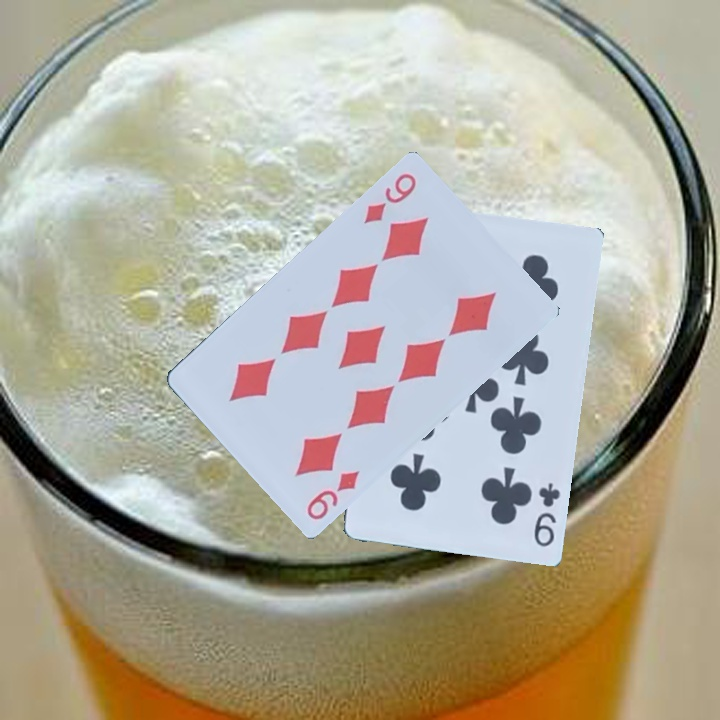
\includegraphics[scale=0.5]{slike/dveKarte}
  \caption{Слика за тренирање која садржи две карте}
  \label{fig:dveKarte}
\end{figure}

Други део тренинг скупа, са три карте поређане као када се држе у руци, се извршава
функцијом \verb create3CardsScene() .
Циљ је да се изврше две трансформације за две карте појединачно, а онда трећа трансформација
све три карте као групе.

На почетку функције \verb create3CardsScene()  се извршавају позиви функције
\verb hull_to_kps()  за полигоне око знака и броја две карте. Праве се нулте матрице
за све три карте, димензија улазне слике, и уписују у атрибуте класе \verb self.img1 ,
\verb self.img2  и \verb self.img3 .
Слике карата, сачуване као матрице у улазним променљивама \verb img1 ,
\verb img2  и \verb img3 , се уписују у наведене нулте матрице на почетним позцијама,
тако да карте пре извршавања трансформација буду у центру слике, а
координате почетне позиције карата за слику са три карте
су дефинисане као:
\begin{minted}{python}
decalX3=int(imgW/2)
decalY3=int(imgH/2-cardH)
\end{minted}

Над \verb self.img3  и \verb self.img2  се позива функција \verb augment()  и прослеђују
трансформације које желимо да извршимо над њима \verb trans_rot1  и \verb trans_rot2 ,
респективно. Уз то се функцији \verb augment()  прослеђују још и „кључне тачке” граничног
оквира око карте \verb cardKP , и изнад добијене „кључне тачке” позивањем
функције \verb hull_to_kps() .
\newpage
\begin{minted}{python}
trans_rot1 = iaa.Sequential([
    iaa.Affine(translate_px={"x": (10, 20)}),
    iaa.Affine(rotate=(22,30)) ])
trans_rot2 = iaa.Sequential([
    iaa.Affine(translate_px={"x": (0, 5)}),
    iaa.Affine(rotate=(10,15)) ])
transform_3cards = iaa.Sequential([
    iaa.Affine(translate_px={"x":decalX-decalX3,"y":decalY-decalY3}),
    iaa.Affine(scale=[0.65,1]),
    iaa.Affine(rotate=(-180,180)),
    iaa.Affine(translate_percent={"x":(-0.2,0.2),"y":(-0.2,0.2)})   
])
\end{minted}

Следи \verb while  петља у којој се извршава трансформација над све три карте, дефинисана
у променљивој \verb transform_3cards . Функција \verb augment()  се позива над
\verb self.img1 , \verb self.img2  и \verb self.img3 .

Изван петље се уписују гранични оквири око знака и броја
у атрибут класе \verb self.listbba , а прослеђују се као инстанце класе \verb BBA .

На крају функције \verb create3CardsScene()  се спајају позадина и три карте у једну слику
и коначна слика је уписана у атрибут класе \verb self.final . На слици \ref{fig:triKarte}
је приказан пример слике са три карте.

\begin{figure}[H]
  \centering
      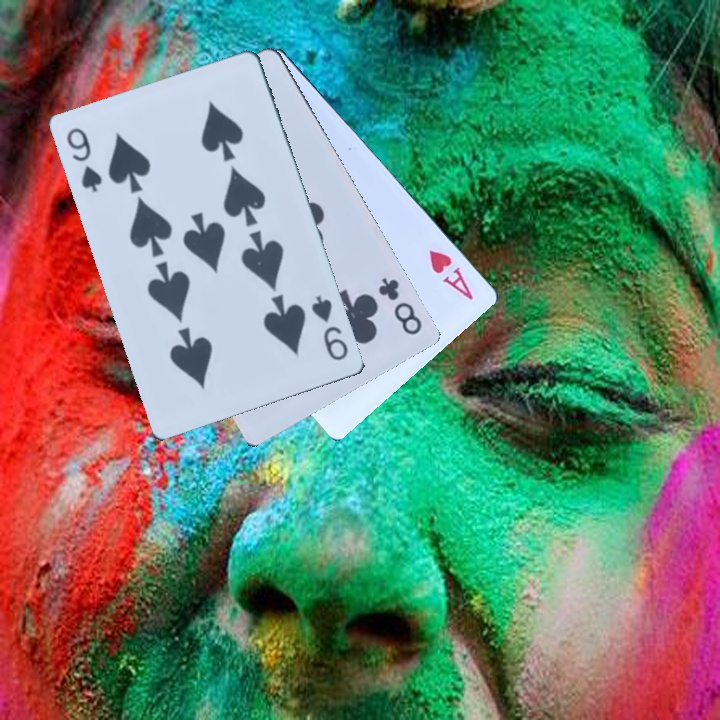
\includegraphics[scale=0.5]{slike/triKarte}
  \caption{Слика за тренирање која садржи три карте}
  \label{fig:triKarte}
\end{figure}

Наредни корак у прављену скупа за тренирање је да се, поред позива функција
\verb create2CardsScene()  и \verb create3CardsScene() , сачува и информација о позицији
знака и броја на слици. 

У следећој „ћелији” кода Jupyter свеске је дефинисан облик
означавања података у XML језику, као и функција \verb create_voc_xml()  која чува
вредности у већ одређеном XML формату. Аргументи функције су излазна XML датотека,
назив слике тј.\ путања и листа граничних оквира око знака и броја.

\begin{minted}{python}
xml_body_1="""<annotation>
        <folder>FOLDER</folder>
        <filename>{FILENAME}</filename>
        <path>{PATH}</path>
        <source>
                <database>Unknown</database>
        </source>
        <size>
                <width>{WIDTH}</width>
                <height>{HEIGHT}</height>
                <depth>3</depth>
        </size>
"""
xml_object=""" <object>
                <name>{CLASS}</name>
                <pose>Unspecified</pose>
                <truncated>0</truncated>
                <difficult>0</difficult>
                <bndbox>
                        <xmin>{XMIN}</xmin>
                        <ymin>{YMIN}</ymin>
                        <xmax>{XMAX}</xmax>
                        <ymax>{YMAX}</ymax>
                </bndbox>
        </object>
"""
xml_body_2="""</annotation>        
"""

def create_voc_xml(xml_file, img_file,listbba,display=False):
    with open(xml_file,"w") as f:
        f.write(xml_body_1.format(**{'FILENAME':os.path.basename(img_file),
		  'PATH':img_file,'WIDTH':imgW,'HEIGHT':imgH}))
        for bba in listbba:            
            f.write(xml_object.format(**{'CLASS':bba.classname,
		'XMIN':bba.x1,'YMIN':bba.y1,'XMAX':bba.x2,'YMAX':bba.y2}))
        f.write(xml_body_2)
        if display: print("New xml",xml_file)
\end{minted}


\subsection{Превођење XML датотека у формат YOLO алгоритма}

Поред Jupyter свеске \verb creating_playing_cards_dataset.ipynb  чији је садржај
изнад описан, у GitHub репозиторијуму наведеном у литератури \cite{git_karte} се налази
и Python датотека \verb convert_voc_yolo.py . Ова датотека омогућава претварање
података о објектима који се налазе на слици из дефинисаног XML формата у
формат који одговара YOLO алгоритму, који ће бити примењен за тренирање.

Жељени формат је
\verb <класа-објекта>  \verb <x>  \verb <y>  \verb <ширина>  \verb <висина> \cite{git_YOLOformat}:
\begin{itemize}
 \item \verb <класа-објекта>  - редни број класе, \verb 0  до \verb (бројКласа-1) {}
 \item \verb <x>  \verb <y>  \verb <ширина>  \verb <висина>  - рационалне вредности релативне
	  у односу на висину и ширину слике, могу имати узети вредност из \verb (0.0,1.0] {}
 \item на пример: \verb <x>  \verb =  \verb <апсолутно_x>  \verb /  \verb <ширина_слике>  или\\
		  \verb <висина>  \verb =  \verb <апсолутна_висина>  \verb /  \verb <висина_слике> {}
 \item \verb <x>  и \verb <y>  - су центар правоугаоника (не горњи-леви ћошак)
\end{itemize}

У датотеци \verb convert_voc_yolo.py  се пролази кроз XML датотеку и налазе потребни подаци,
а кључна функција за превођење у YOLO формат је \verb convert() .
У аргументу \verb size  се налазе димензије слике, а у \verb box  су садржане \verb x  и
\verb y  координате ћошкова граничног оквира око знака и броја карте.

С обзиром да \verb <x>  и \verb <y>  у жељеном формату представљају центар оквира
тј.\ правоугаоника, те
вредности се добијају аритметичком средином улазних. Дељењем са ширином тј.\ висином
слике се добијају релативне вредности.

\begin{minted}{python}
def convert(size, box):
    dw = 1./size[0]
    dh = 1./size[1]
    x = (box[0] + box[1])/2.0
    y = (box[2] + box[3])/2.0
    w = box[1] - box[0]
    h = box[3] - box[2]
    x = x*dw
    w = w*dw
    y = y*dh
    h = h*dh
    return (x,y,w,h)
\end{minted}

\newpage
\section{Вештачке неуронске мреже - теорија}

\subsection{Увод у вештачке неуронске мреже}
\textbf{Неурон} је основна јединица вештачке неуронске мреже и има своје улазе,
над којима извршава рачунске операције и добијену вредност уписује
као излаз \cite{nn_osnova}. Овако изгледа неурон са два улаза:

\begin{figure}[H]
  \centering
      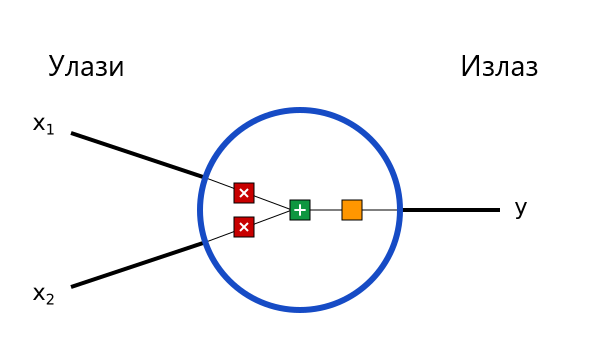
\includegraphics[scale=0.5]{slike/neuron}
  \caption{Неурон}
  \label{fig:neuron}
\end{figure}

Одигравају се три ствари. Прво се улази $x_1$ и $x_2$ множе тежинама
веза $w_1$ и $w_2$, па се сви ови производи сабирају
и том збиру додаје и праг активације $b$.
На крају се ова вредноста проследи активационој функцији и добија се излазна вредност.

\begin{equation}
 y = f(x_1 * w_1 + x_2 * w_2 + b)
\end{equation}

Функција која се често примењује као активациона је Сигмоидна функциja,
дефинисана као $S(x) = \frac{1}{1+e^{-x}}$.

\begin{figure}[H]
  \centering
      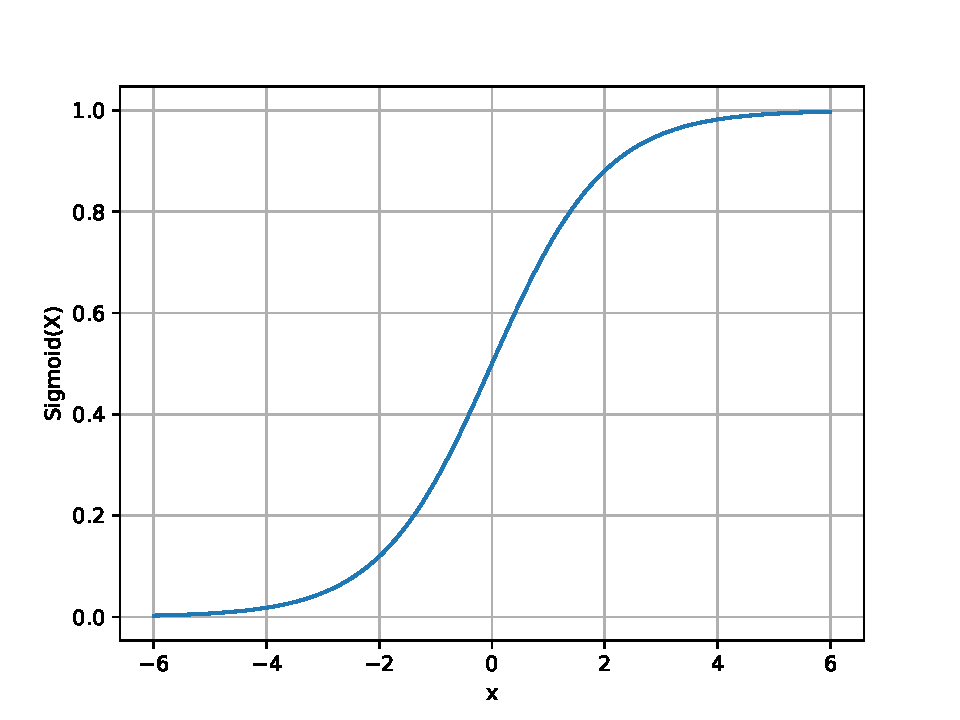
\includegraphics[scale=0.5]{slike/sigmoid}
  \caption{Сигмоидна функција}
  \label{fig:sigmoid}
\end{figure}

Ако би тежине веза имале вредности $w_1 = 0$ и $w_2 = 1$ тј.\ $w=[0,1]$
(ако се представе као вектор),
праг активације $b = 4$, а
улази неурона $x_1 = 2$ и $x_2 = 3$ ($x=[2,3]$), тада се применом
изнад дефинисане формуле долази до вредности излаза:

\begin{equation}
\begin{split}
(w \cdot x + b) & = ((w_1 * x_1) + (w_2 * x_2)) + b \\
& = 0 * 2 + 1 * 3 + 4 \\
& = 7
\end{split}
\end{equation}

\begin{equation}
y = f(w \cdot x + b) = f(7) = 0.999
\end{equation}
Када улази неурона износе $x=[2,3]$, излазна вредност је $0.999$.
Овакав процес прослеђивања улазних вредност напред назива се \textbf{пропагација унапред}.

\textbf{Неуронска мрежа} је скуп међусобно повезаних неурона. На слици
\ref{fig:neuronskaMreza} је приказан пример вештачке неуронске мреже:

\begin{figure}[H]
  \centering
      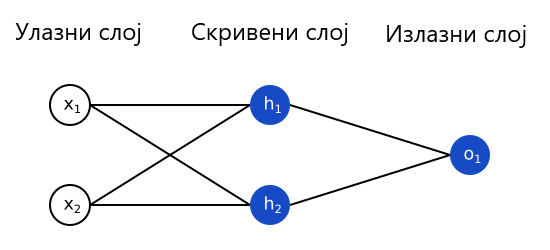
\includegraphics[scale=0.6]{slike/neuronskaMreza}
  \caption{Вештачка неуронска мрежа}
  \label{fig:neuronskaMreza}
\end{figure}

Ова мрежа има два улаза, скривени слој са два неурона ($h_1$ и $h_2$) и
излазни слој који се састоји од једног неурона $o_1$. \textbf{Скривени слој}
је било који слој између улазног и излазног слоја и могуће је да се
вештачка неуронска мрежа састоји од много скривених слојева.

Претпоставимо да сви неурони имају исте тежине веза
$w_1 = 0$ и $w_2 = 1$ тј.\ $w = [0,1]$, исти праг активације $b = 0$ и
сви неурони као активациону функцију користе Сигмоидну функцију; тада
се следећим рачуном добија излазна вредност, ако се на улаз проследи
вредност $x=[2,3]$:

\begin{equation}
\begin{split}
h_1 = h_2 & = f(w \cdot x + b) \\
& = f((0 * 2) + (1 * 3) + 0) \\
& = f(3) \\
& = 0.9526
\end{split}
\end{equation}

\begin{equation}
\begin{split}
o_1 & = f(w \cdot [h_1, h_2] + b) \\
& = f((0 * h_1) + (1 * h_2) + 0) \\
& = f(0.9526) \\
& = 0.7216
\end{split}
\end{equation}

Вештачка неуронска мрежа може да има произвољан број слојева и неурона у њима.

Користимо следеће податке за пример тренирања вештачке неуронске мреже:
\begin{table}[ht]
\centering
 \begin{tabular}{| c | c | c | c |}
  \hline
  Име & Тежина (lb) & Висина (in) & Пол \\
  \hline
  Наташа & 133 & 65 & Ж\\
  Бајага & 160 & 72 & М\\
  Ђоковић & 152 & 70 & М\\
  Ивана & 120 & 60 & Ж\\
  \hline
 \end{tabular}
 \caption{Пример тренинг скупа података}
\end{table}

Сада следи тренирање мреже која треба да предвиди пол особе, а као
улазне параметре има тежину и висину:

\begin{figure}[H]
  \centering
      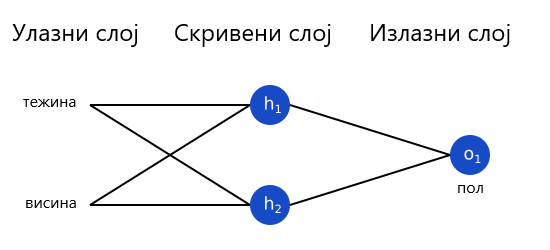
\includegraphics[scale=0.6]{slike/neuronskaMrezaTren.png}
  \caption{Вештачка неуронска мрежа која треба да се тренира}
  \label{fig:nn_osnovaTren}
\end{figure}

У наредној табели су \textit{Мушкарци} означени бројем 0, \textit{Жене} бројем 1, a
остале вредности су подједнако смањене, да би израчунавање било једноставније:

\begin{table}[ht]
\centering
 \begin{tabular}{| c | c | c | c |}
  \hline
  Име & Тежина (минус 135) & Висина (минус 66) & Пол \\
  \hline
  Наташа & -2 & -1 & 1\\
  Бајага & 25 & 6 & 0\\
  Ђоковић & 17 & 4 & 0\\
  Ивана & -15 & -6 & 1\\
  \hline
 \end{tabular}
 \caption{Умањене вредности (припрема тренинг скупа)}
\end{table}


Тренирање мреже је побољшање тачности предвиђања мреже. Да би се тачност повећала потребно
је имати некакву мерило, па се
дефинишу термини \textbf{функција губитка} $L$ (Loss function) и
\textbf{функција трошка} $J$ (Cost function). Функција губитка се односи на један пример тренинг
скупа, док је функција трошка средња вредност извршених функција губитка над свим
примерима скупа, уз додатну „регуларизацију” \cite{stackex_loss}.
\newpage
Нека је на пример \textit{средња квадратна грешка} (\textit{mean square error}) функција трошка:
\begin{equation}
J = MSE = \frac{1}{m} \sum_{i=1}^{m} (y_{true} - y_{pred})^2
\end{equation}
Где је:
\begin{itemize}
 \item $m$ је број примера тј.\ 4 (Наташа, Ђоковић, Бајага, Ивана)
 \item $y$ је променљива коју треба да предвидимо тј.\ Пол
 \item $y_{true}$ је „тачан одговор”. На пример, $y_{true}$ за Наташу би био 1 (\textit{Жена}).
 \item $y_{pred}$ је вредност коју смо предвидели, оно што је излаз неуронске мреже
\end{itemize}

Предвиђање је боље, уколико је функција трошка мања, па је
\textbf{тренирање мреже поступак промене вредности тежине веза и
прагова активације са циљем да се одреди што нижа функција трошка}.

Нека мрежа увек као излаз даје $0$ тј.\ увек предвиђа да је особа \textit{Мушкарац};
онда функција трошка тј.\ \textit{средња квадратна грешка} износи:
\begin{table}[ht]
\centering
 \begin{tabular}{| c | c | c | c |}
  \hline
  Име & $y_{true}$ & $y_{pred}$ & $(y_{true} - y_{pred})^2$ \\
  \hline
  Наташа & 1 & 0 & 1\\
  Бајага & 0 & 0 & 0\\
  Ђоковић & 0 & 0 & 0\\
  Ивана & 1 & 0 & 1\\
  \hline
 \end{tabular}
 \caption{Вредности функције губитка}
 \label{tab:primerSkupa}
\end{table}

\begin{equation}
MSE = \frac{1}{4} (1 + 0 + 0 + 1) = 0.5
\end{equation}

Нека се сада скуп састоји само из једног примера тј.\ особе:
\begin{table}[ht]
 \centering
 \begin{tabular}{| c | c | c | c |}
  \hline
  Име & Тежина (минус 135) & Висина (минус 66) & Пол \\
  \hline
  Наташа & -2 & -1 & 1\\
  \hline
 \end{tabular}
 \caption{Скуп који се састоји од једне \textit{особе}}
 \label{tab:natasa}
\end{table}

Средња квадратна грешка сада износи:
\begin{equation}
\begin{split}
MSE & = \frac{1}{1} \sum_{i=1}^{1} (y_{true} - y_{pred})^2 \\
& = (y_{true} - y_{pred})^2 \\
& = (1 - y_{pred})^2
\end{split}
\end{equation}
\newpage
На слици \ref{fig:nn_osnovaOznake} су означене ознаке тежине веза
и прагови активације:
\begin{figure}[H]
  \centering
      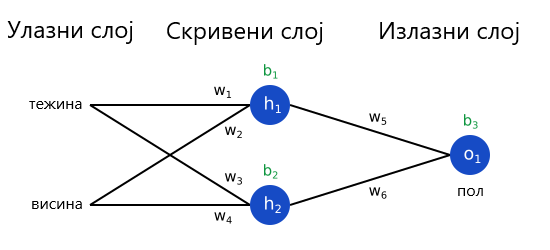
\includegraphics[scale=0.6]{slike/neuronskaMrezaOznake.png}
  \caption{Тежине веза и прагови активације у вештачкој неуронској мрежи}
  \label{fig:nn_osnovaOznake}
\end{figure}

Функција трошка може да се представи као функција 
са више променљивих:
\begin{equation}
Ј(w_1,w_2,w_3,w_4,w_5,w_6,b_1,w_2,w_3)
\end{equation}
Промена вредности $w_1$, мења вредност $Ј$, па је потребно израчунати
парцијални извод. Парцијални извод је представљен као:

\begin{equation}
\frac{\partial J}{\partial w_1} = \frac{\partial J}{\partial y_{pred}} * \frac{\partial y_{pred}}{\partial w_1}
\end{equation}

Изнад је већ добијена вредност $J = (1 - y_{pred})^2$, па је могуће израчунати
$\partial J / \partial y_{pred}$:
\begin{equation}
\frac{\partial L}{\partial y_{pred}} = \frac{\partial (1 - y_{pred})^2}{\partial y_{pred}} = -2(1 - y_{pred})
\end{equation}

Потребно је одредити $\partial y_{pred} / \partial w_1$ и као у изнад
наведеном примеру пропагације унапред, $h_1$, $h_2$ и $o_1$ су излази
одговарајућих неурона. Тада је
\begin{equation}
y_{pred} = o_1 = f(w_5 h_1 + w_6 h_2 + b_3),
\end{equation}
где је $f$ Сигмоидна функција.

Пошто $w_1$ утиче на $h_1$ (не $h_2$), може се написати
\begin{equation}
\begin{gathered}
\frac{\partial y_{pred}}{\partial w_1} = \frac{\partial y_{pred}}{\partial h_1} * \frac{\partial h_1}{\partial w_1} \\
\frac{\partial y_{pred}}{\partial h_1} = w_5 * f'(w_5 h_1 + w_6 h_2 + b_3)
\end{gathered}
\end{equation}

Урађено је исто и за $\partial h_1 / \partial w_1$:
\begin{equation}
\begin{gathered}
h_1 = f(w_1 x_1 + w_2 x_2 + b_1) \\
\frac{\partial h_1}{\partial w_1} = x_1 * f'(w_1 x_1 + w_2 x_2 + b_1),
\end{gathered}
\end{equation}

где је $x_1$ улаз неурона који представља тежину особе, а $x_2$ висину.

Извод Сигмоидне функције је:
\begin{equation}
\begin{gathered}
f(x) = \frac{1}{1 + e^{-x}} \\
f'(x) = \frac{e^{-x}}{(1 + e^{-x})^2} = f(x) * (1 - f(x))
\end{gathered}
\label{eq:izvod}
\end{equation}

Сада је парцијални извод сведен на чланове које је могуће израчунати:
\begin{equation}
\frac{\partial J}{\partial w_1} = \frac{\partial J}{\partial y_{pred}} * \frac{\partial y_{pred}}{\partial h_1} * \frac{\partial h_1}{\partial w_1}
\end{equation}

Поступак рачунања парцијалних извода идући од излаза ка улазу
вештачке неуронске мреже
назива се \textbf{пропагација уназад}.

Над скупом са једном \textit{особом}, приказаним у табели \ref{tab:natasa},
ће бити израчунати парцијални изводи.

Иницијализоване су вредности тежине веза на 1, а прагови активације на 0. Ако
се изврши пропагација унапред, добија се:
\begin{equation}
\begin{gathered}
\begin{split}
h_1 & = f(w_1 x_1 + w_2 x_2 + b_1) \\
& = f(-2 + -1 + 0) \\
& = 0.0474
\end{split}\\

\begin{split}
h_2 = f(w_3 x_1 + w_4 x_2 + b_2) = 0.0474
\end{split}\\

\begin{split}
o_1 & = f(w_5 h_1 + w_6 h_2 + b_3) \\
& = f(0.0474 + 0.0474 + 0) \\
& = 0.524
\end{split}
\end{gathered}
\end{equation}

Излаз мреже има вредност $y_{pred}=0.524$, а то је вредност која
не указује јасно да ли је \textit{особа} \textit{Мушкарац} ($0$)
или \textit{Жена} ($1$).

Сада ће бити израчунато
\footnote{\label{izvod} Извод $f'(x) = f(x) * (1-f(x))$ за Сигмоидну функцију
је израчунат у једначини (\ref{eq:izvod}).}
$\partial J / \partial w_1$:
\begin{equation}
\begin{gathered}
\begin{split}
\frac{\partial J}{\partial w_1} = \frac{\partial J}{\partial y_{pred}} * \frac{\partial y_{pred}}{\partial h_1} * \frac{\partial h_1}{\partial w_1}
\end{split} \\
\begin{split}
\frac{\partial J}{\partial y_{pred}} & = -2 (1 - y_{pred}) \\
& = -2 (1 - 0.524) \\
& = -0.952
\end{split}\\
\begin{split}
\frac{\partial y_{pred}}{\partial h_1} & = w_5 * f'(w_5 h_1 + w_6 h_2 + b_3) \\
& = 1 * f'(0.0474 + 0.0474 + 0) \\
& = f(0.0948) * (1- f(0.0948)) \\
& = 0.249
\end{split} \\
\begin{split}
\frac{\partial h_1}{\partial w_1} & = x_1 * f'(w_1 x_1 + w_2 x_2 + b_1) \\
& = -2 * f'(-2 + -1 + 0) \\
& = -2 * f(-3) * (1 - f(-3)) \\
& = -0.0904
\end{split} \\
\begin{split}
\frac{\partial J}{\partial w_1} & = -0.952 * 0.249 * -0.0904 \\
& = 0.0214
\end{split}
\end{gathered}
\end{equation}

Може се закључити да би се вредност функције трошка $Ј$ врло мало повећала,
уколико би $w_1$ било повећано.

Следи тренирање мреже и биће коришћен алгоритам
\textit{Стохастички градијентни спуст} којим се одређује како
мењати вредности тежина веза и прагова активације, да би се
минимизовала вредност функције трошка $J$.

Представљен је следећом једначином:
\begin{equation}
w_1 \leftarrow w_1 - \eta \frac{\partial J}{\partial w_1},
\label{eq:osnoveGradSpust}
\end{equation}
где је $\eta$ константа и представља \textbf{дужину корака при учењу}
(\textbf{learning rate}),
њиме се контролише колико брзо учимо. Одузима се $\eta \frac{\partial J}{\partial w_1}$
од $w_1$:
\begin{itemize}
 \item ако је $\partial J / \partial w_1$ позитивно, $w_1$ ће се
  смањити, па ће се и $J$ смањити
 \item ако је $\partial J / \partial w_1$ негативно, $w_1$ ће се
  повећати, па ће се и $J$ смањити
\end{itemize}
Ако се ово уради над свим тежинама веза и праговима активације
(у једначини (\ref{eq:osnoveGradSpust}) се $b_1$ замени уместо $w_1$),
функција трошка ће се смањивати тј.\ неуронска мрежа ће се побољшавати.

\newpage
\subsection{Конволуцијске неуронске мреже}
Рачунарски вид (Computer vision) је грана која се изузетно брзо развија.
Примена ове области је веома широка: детекција пешака и других аутомобила
током аутономне вожње, препознавање лица примењено на откључавање телефона или
врата, препознавање врсте хране итд.\ \cite{ngCVision}.

Један од проблема у овој области је да подаци (слике) на улазу могу да буду велики.
На пример, над сликом \ref{fig:macka} је потребно извршити класфикацију да ли се на њој
налази мачка или не, а на излазу се добија вредност 0 или 1.

\begin{figure}[H]
  \centering
      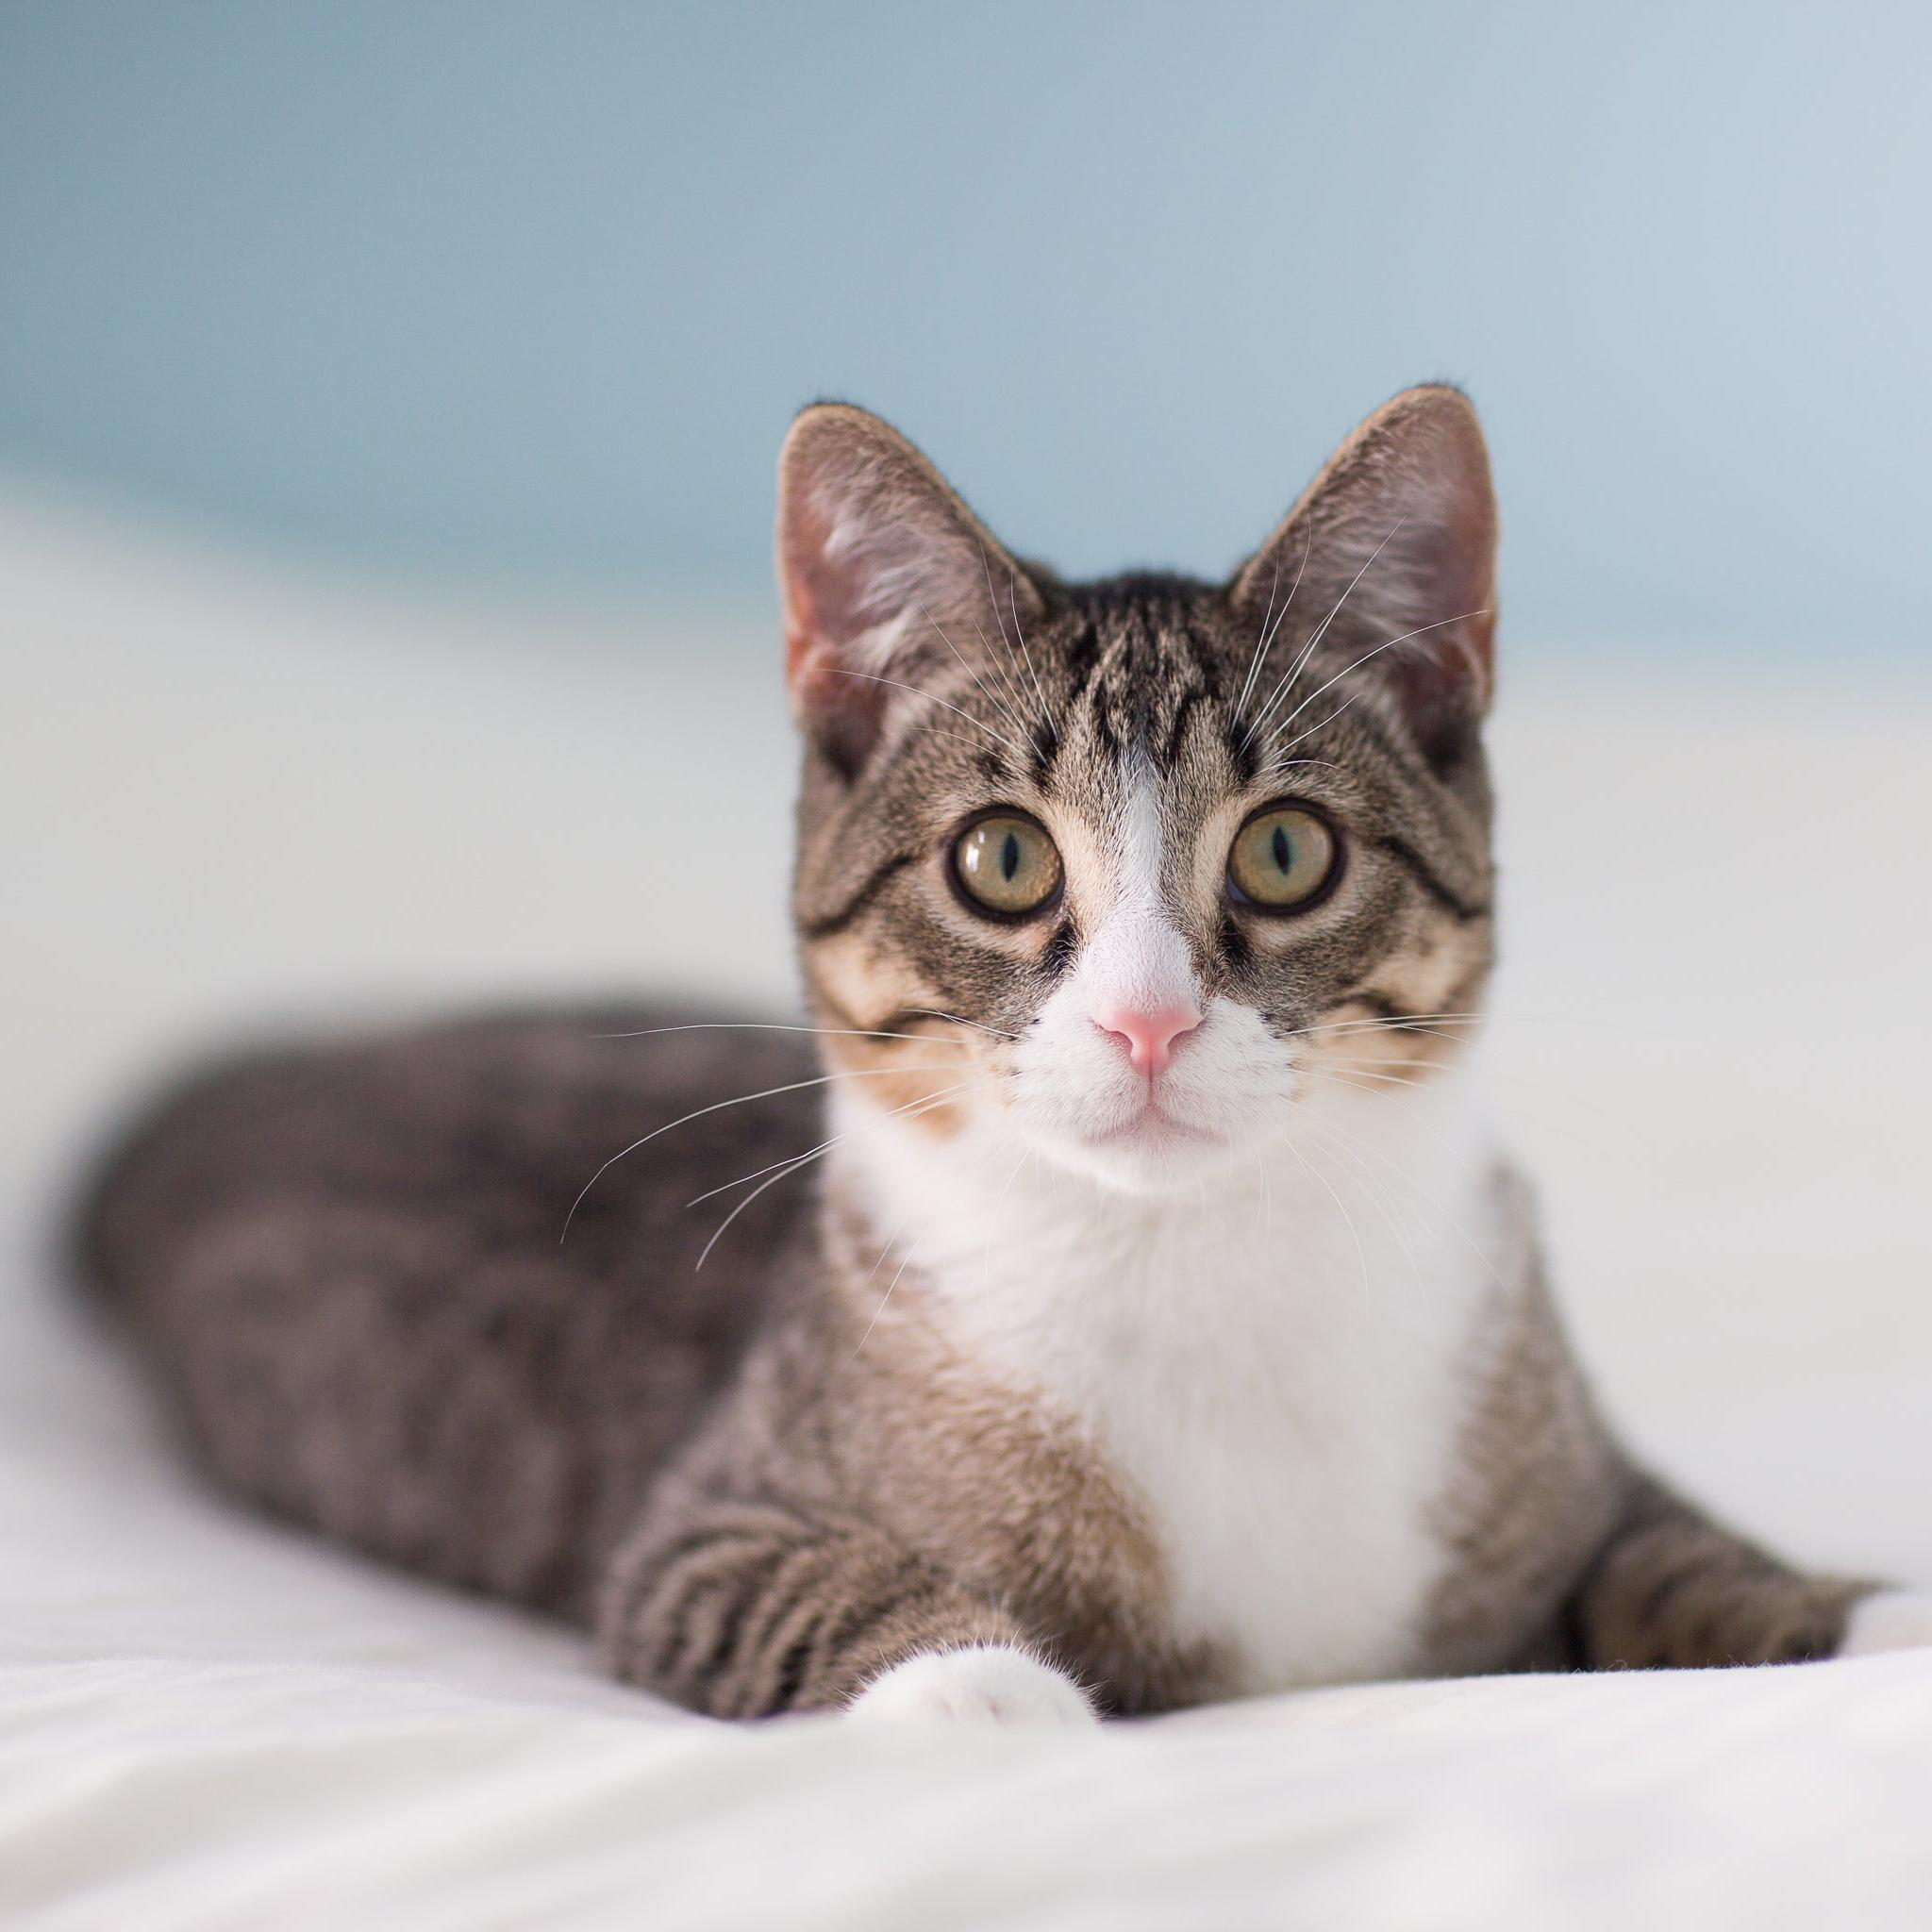
\includegraphics[scale=0.2]{slike/macka.jpg}
  \caption{Слика великих димензија на улазу у мрежу}
  \label{fig:macka}
\end{figure}

Уколико је слика \ref{fig:macka} димензија $1000 \times 1000 \times 3$
(последња димензија 3 односи на три основне боје
које се налазе у пикселу: црвену, зеленy и плавy),
то значи да је величина улазних података 3000000.
\newpage
Слика \ref{fig:ng_FCVision}
приказује неуронску мрежу којој је прослеђена слика наведених димензија, па
ако се претпостави да први слој има 1000 неурона, то значи да би само матрица
тежина веза између прва два слоја имала димензије (1000,3000000), а тада израчунавање
постаје неизводљиво.

\begin{figure}[H]
  \centering
      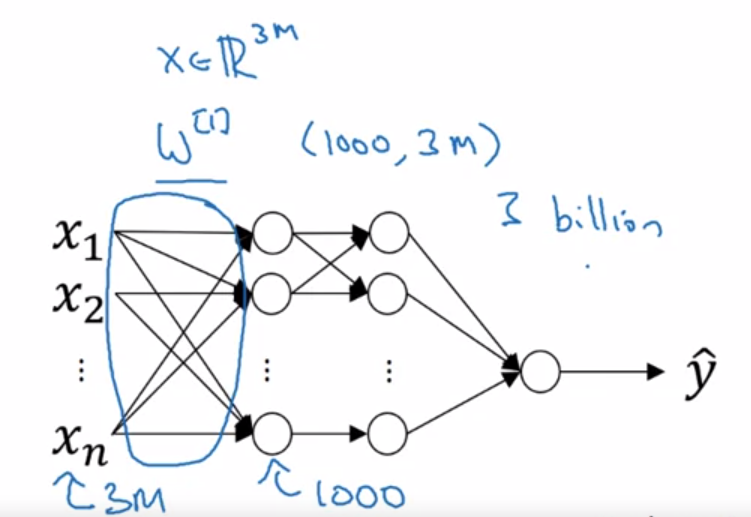
\includegraphics[scale=0.45]{slike/ngFCVision.png}
  \caption{Превелика величина података на улазу у мрежу}
  \label{fig:ng_FCVision}
\end{figure}

Операција \textbf{конволуције} је једна од основа за прављење конволуцијске
неуронске мреже. Извршавање операције је приказано следећом сликом и на њој се
види да се на улазу налази улазна матрица димензија $6\times6$ и над њом
се изршава конволуција применом $3\times3$ филтера, да би се на излазу нашла матрица
димензија $4\times4$.

\begin{figure}[H]
  \centering
      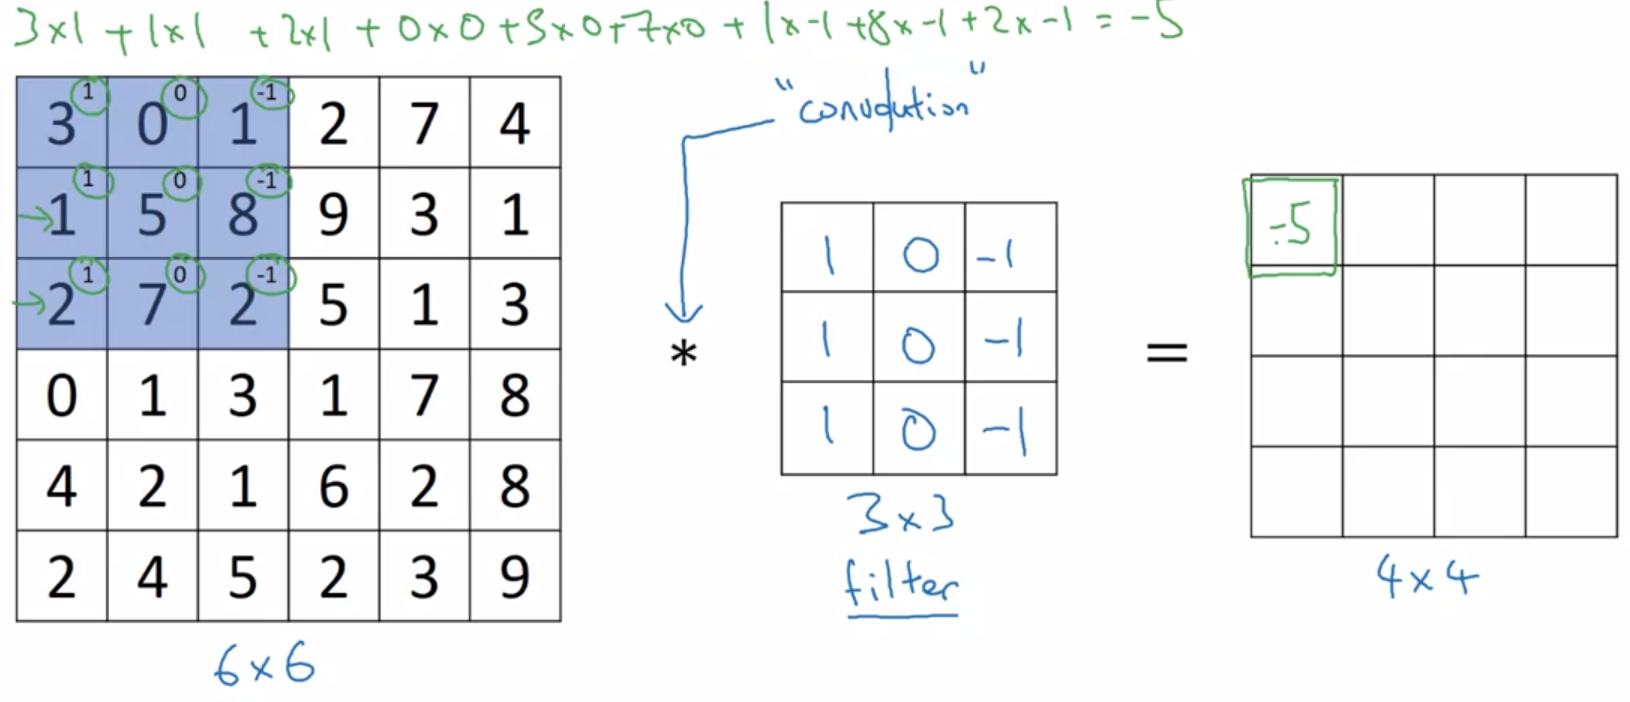
\includegraphics[scale=0.35]{slike/ngKonvoucija.png}
  \caption{Операција конволуције}
  \label{fig:ng_Kovolucija}
\end{figure}

Операција се извршава тако што је вредност поља (1,1) у излазној матрици,
једнак збиру производа
чланова исечка (димензија филтера), улазне матрице и чланова филтера. Исечак
(димензија филтера) се помера једно поље у страну (односно у следећи ред) и
извршава се исти поступак.

Кроз пример \textit{детектовања ивица} ће бити објашњен рад конволуцијске
неуронске мреже \cite{ngEdgeDet}.

Применом много сложенијих неуронских мрежа у односу на оне које су приказане
у претходном потпоглављу, могуће је решити проблем детекције лица. Први
слојеви би детектовали \textit{прелазе боја} (\textit{ивице}), средњи
слојеви налазе делове лица (очи, нос \dots), док би виши слојеви
на основу тих информација налазили лица.

Сада ће бити објашњено решавање првог случаја детекције ивица
са слике \ref{fig:ng_Edge1}, применом конволуцијских неуронских мрежа.

\begin{figure}[H]
  \centering
      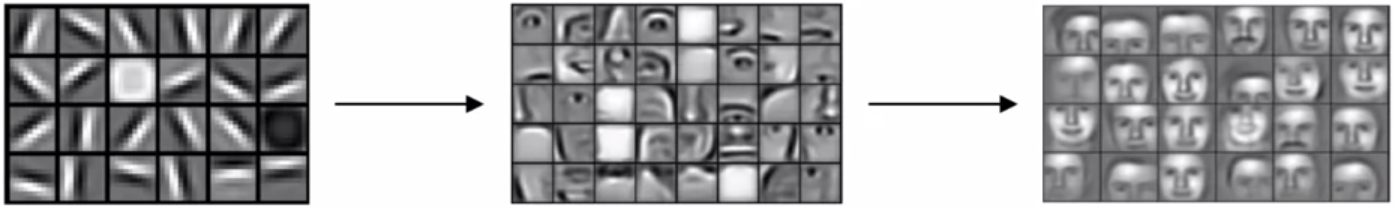
\includegraphics[scale=0.4]{slike/ngEdge1.png}
  \caption{Поступак детекције лица}
  \label{fig:ng_Edge1}
\end{figure}

Нека је задатак да се детектују \textit{вертикалне ивице}, а на улазу се
налази једноставна матрица.
Слика \ref{fig:ng_KonvoucijaVert} приказује
извршену операцију конволуције. Веће вредности у матрицама се односе
на јаче осветљење пиксела, па се на излазу види да је у средини 
светлије, а са стране тамније, што се чита као
вертикални прелаз \textbf{светло-у-тамно}.

\begin{figure}[H]
  \centering
      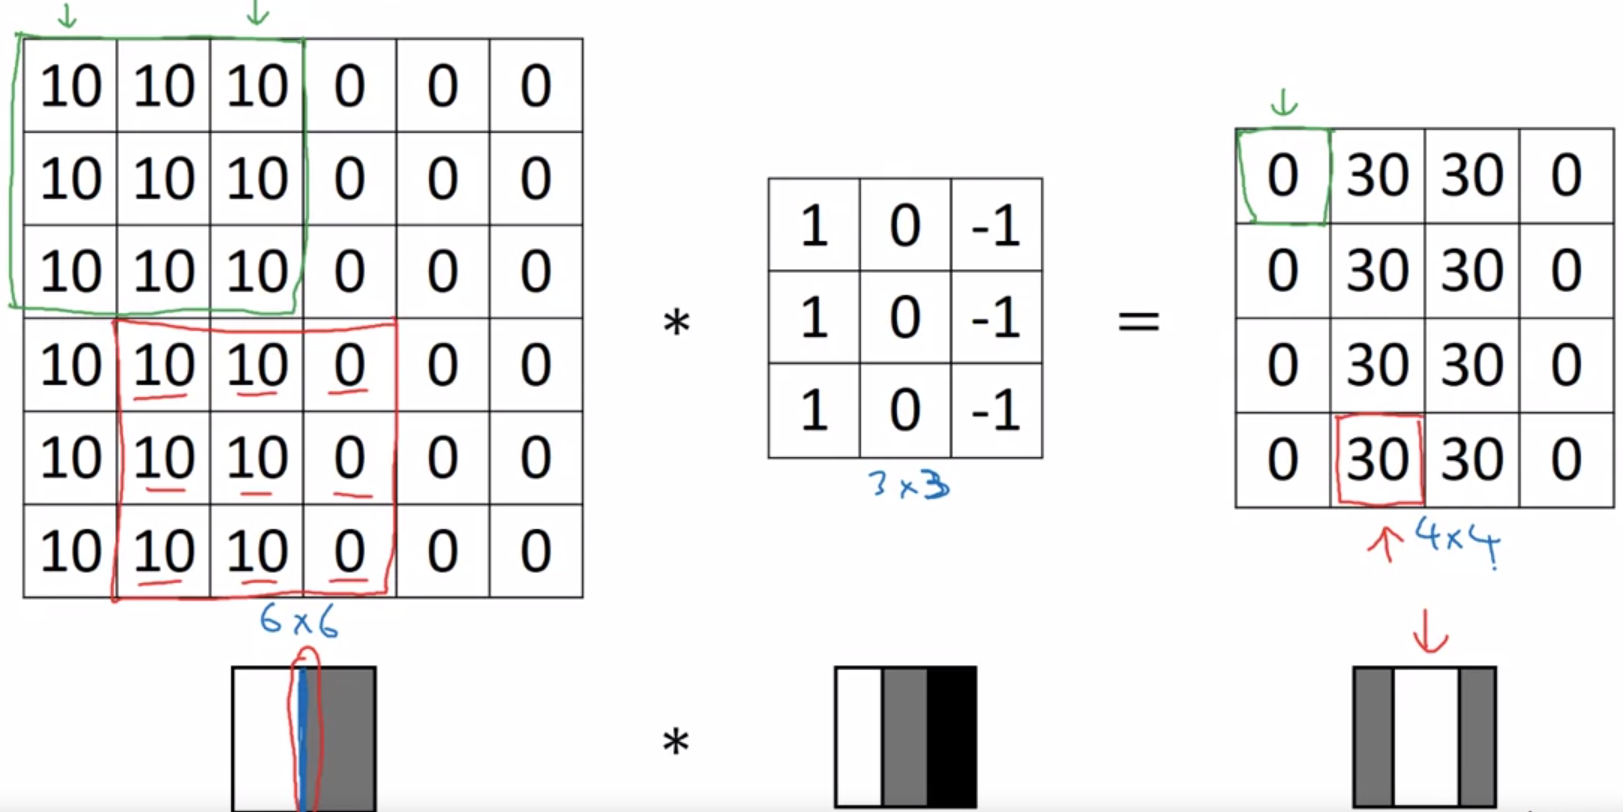
\includegraphics[scale=0.35]{slike/ngKonvoucijaVert.png}
  \caption{Вертикална ивица, прелаз светло-у-тамно}
  \label{fig:ng_KonvoucijaVert}
\end{figure}

Уколико би се на улазу уместо матрице где је светлија лева половина, 
нашла матрица која представља слику ивице где је десна страна светлија, излазна
слика (после конволуције) би имала тамнији део у средини, а на крајевима
би била светлија.
\newpage
Поента је да је извршавањем конволуције коришћењем различитих филтера могуће
детектовати различите ивице.

\textit{С обзиром да постоји много различитих ивица, а њихова детекција се врши
применом различитих филтера тј. вредности поља матрице филтера су различите,
могуће их је посматрати као параметре које је потребно
проследити мрежи на тренирање} \cite{ngMoreEdge}.

\begin{equation}
\begin{bmatrix}
 w_1 & w_2 & w_3 \\
 w_4 & w_5 & w_6 \\
 w_7 & w_8 & w_9
\end{bmatrix}
\label{eq:KonvMatrica}
\end{equation}

При извршавању конволуције је могуће да исечак улазне матрице много пута
покрије поља која се налазе у средини матрице, а само једном „посети” поља
на ивици.

Уводи се \textbf{допуњавање матрице} (\textbf{padding}), а то је поступак
проширивања матрице, чиме се добија да исечак, који се помера за један
корак, посети поља на ивици више пута него пре допуне.

Овом техником се решавају два проблема и постиже се:
\begin{itemize}
 \item да се на излазу нађе мање информација које се односе на средину матрице (слике)
 \item чување информацијa из поља са ивице слике
\end{itemize}

Поља којим се проширује матрицa имају вредност 0, па не утичу на резултат.
\begin{equation}
\begin{bmatrix}
 0 & 0 & 0 & 0 & 0 & 0 & 0 \\
 0 &   &   &   &   &   & 0 \\
 0 &   &   &   &   &   & 0 \\
 0 &   &   &   &   &   & 0 \\
 0 &   &   &   &   &   & 0 \\
 0 &   &   &   &   &   & 0 \\
 0 & 0 & 0 & 0 & 0 & 0 & 0
\end{bmatrix}
\label{eq:KonvMatricaPadd}
\end{equation}
\newpage
Још једна техника, којом се добија излазна матрица мањих димензија, је
\textbf{Конволуција са већим кораком} (\textbf{Strided convolution}) и
разликује се у \textit{кораку} (\textit{stride}) који исечак прави
кроз улазну матрицу.

\begin{figure}[H]
  \centering
      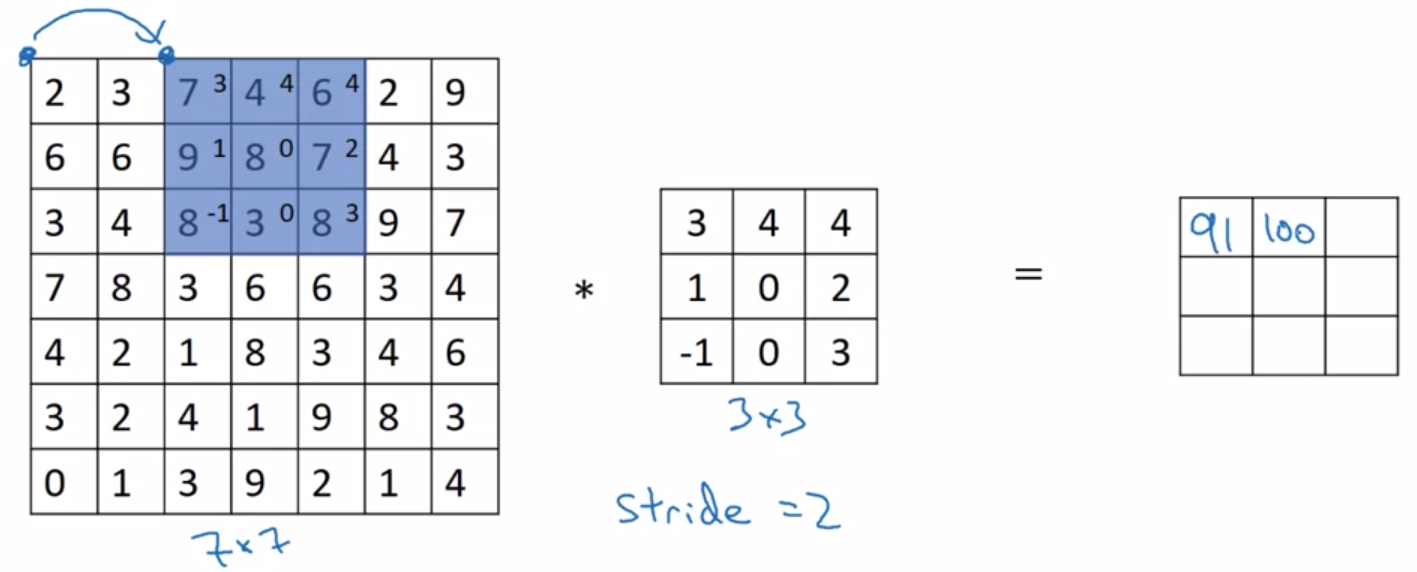
\includegraphics[scale=0.35]{slike/ngConvStride1.png}
  \caption{Конволуција са већим кораком исечка}
  \label{fig:ng_ConvStride1}
\end{figure}

Уколико се на улазу нађе слика димензија $n \times n$ и треба
извршити конволуцију коришћењем филтера димензија $f \times f$, где је
\textit{корак} (\textit{stride}) $s$, а \textit{допуна} (\textit{padding}) $p$;
тада је димензија излазне матрице:
\begin{equation*}
 \floor*{\frac{n+2p-f}{s}+1} \times \floor*{\frac{n+2p-f}{s}+1}
\end{equation*}

Слика \ref{fig:ng_ConvLay1} приказује један слој конволуцијске неуронске
мреже. На излазу се налази активациона функција ReLU, дефинисана као:
\begin{equation}
f(x) = max(0,x),
\end{equation}
а приказана је на наредној слици:

\begin{figure}[H]
  \centering
      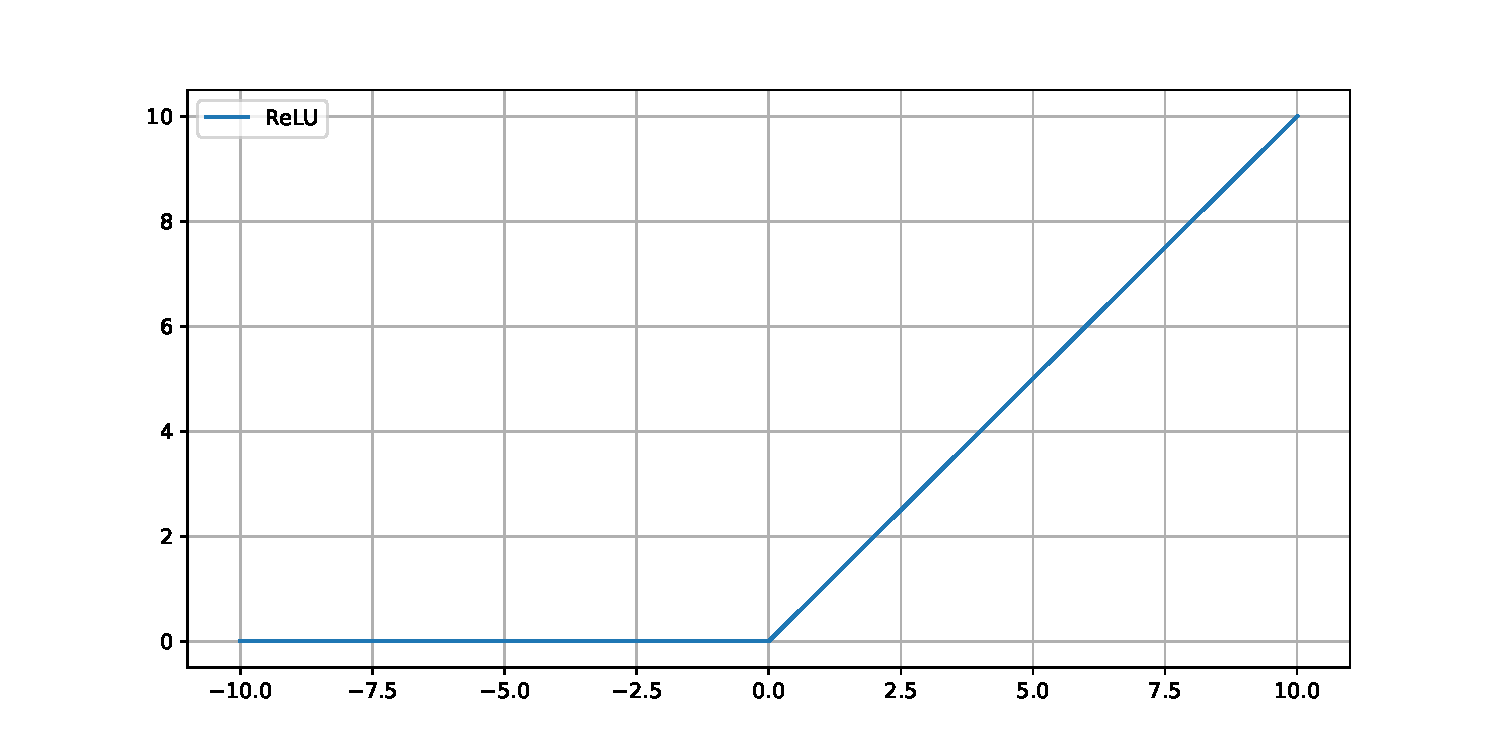
\includegraphics[scale=0.35]{slike/ReLU.pdf}
  \caption{ReLU функција}
  \label{fig:ReLU}
\end{figure}

У примеру се на улазу налазе три матрице и показују вредности
црвене, зелене и плаве боје у пикселима. 

Извршавају се две конволуције
применом два разчичита филтера, а ReLU активационој функцији се прослеђује
резултат конволуције увећан за праг активације.
На излазу се налази матрица димензија $4 \times 4 \times 2$.

\begin{figure}[H]
  \centering
      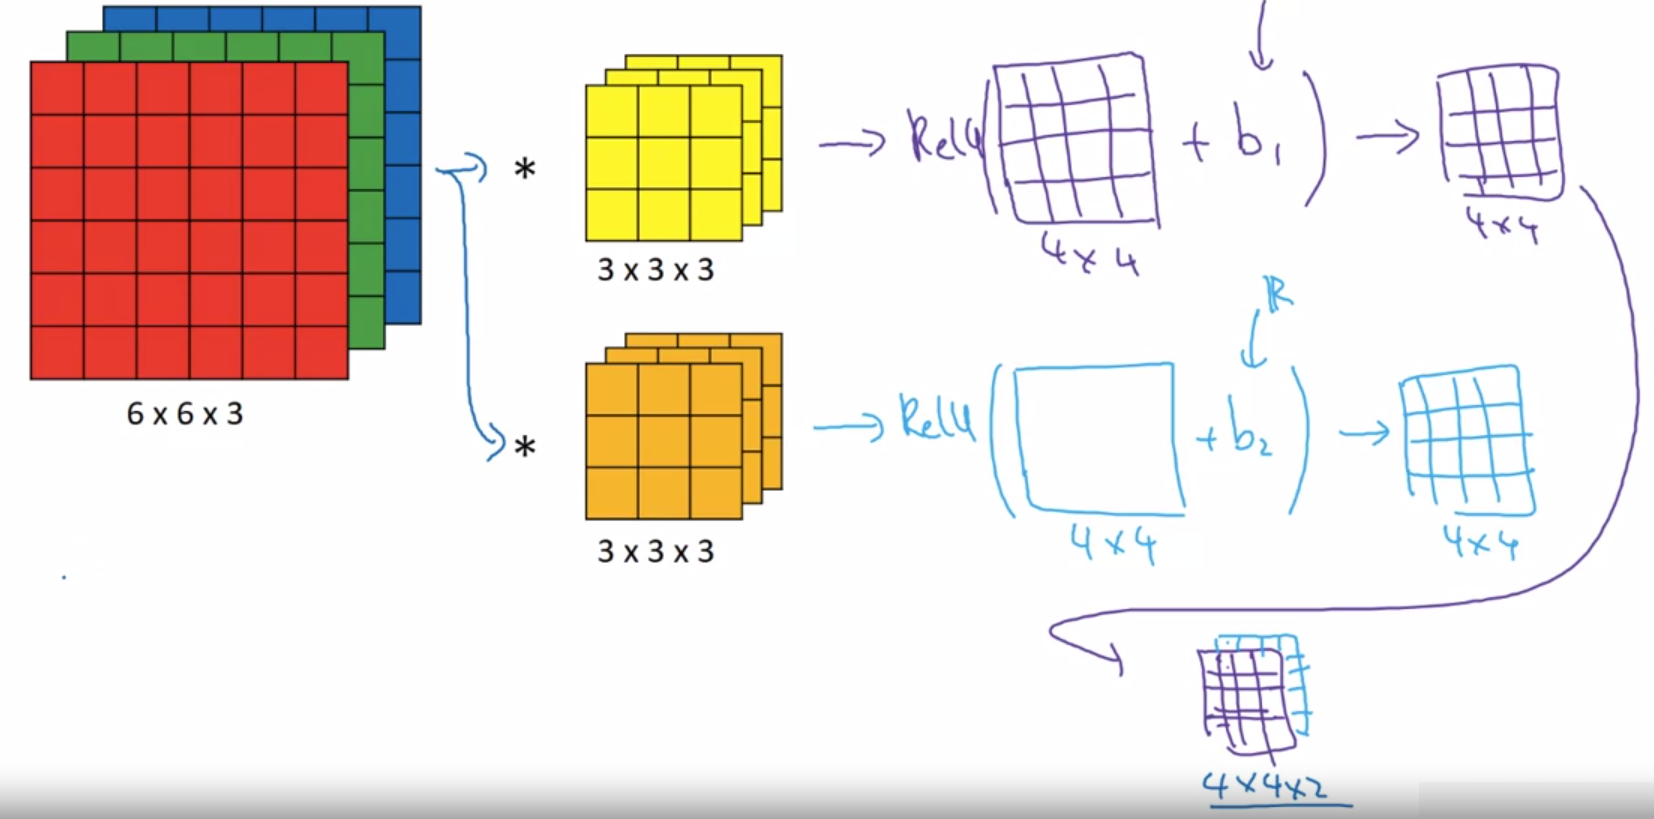
\includegraphics[scale=0.34]{slike/ngConvLay1.png}
  \caption{Пример слоја конволуцијске неуронске мреже}
  \label{fig:ng_ConvLay1}
\end{figure}

\textbf{Оно што је битно да се примети је да колико год да је слика велика,
број параметара за тренирање је дефинисан димензијама филтера, јер
су то вредности које се прилагођавају} \cite{ngConvOneLay}.

На пример, ако постоји 10 филтера димензија $3 \times 3 \times 3$
(27 параметара) и праг активације $b$ за сваки, значи да постоји укупно
280 параметара за тренирање, \textit{без обзира на димензије слике на улазу}!

Врло често је матрица на излазу веома велика и можда ју је потребно
смањити, а да притом главне \textit{одлике} буду сачуване.
Ово се постиже \textbf{Слојевима удруживања} (\textbf{Pooling layers}) и
слика \ref{fig:ng_MaxPool} приказује један тип који се назива
\textit{Удруживање максимума} (\textit{Max pooling}).

\begin{figure}[H]
  \centering
      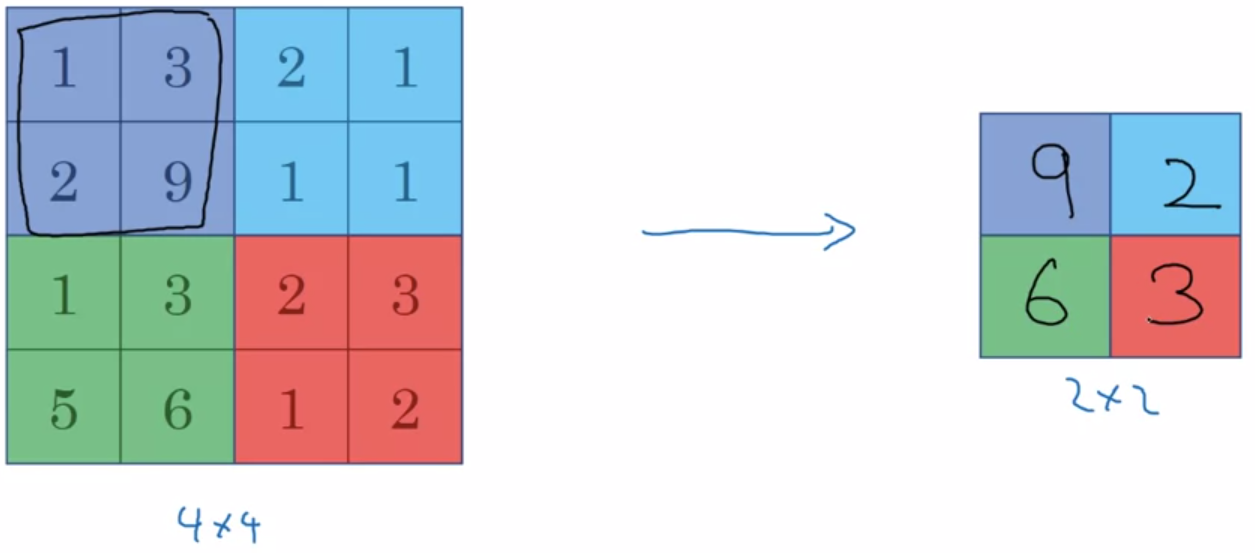
\includegraphics[scale=0.29]{slike/ngMaxPool.png}
  \caption{Max pooling}
  \label{fig:ng_MaxPool}
\end{figure}
Процедура је слична као
и са конволуцијом, јер се дефинише димензија филтера тј.\ исечка $f$ и величина
корака (stride) $s$.

\textit{Удруживање максимума} се разликује од конволуције по томе што сада нема
параметара које треба тренирати, него је опeрација фиксна. \textbf{Максимална
вредност у исечку се уписује у излазну матрицу}.

Идеја је да уколико постоји већа вредност која указује на неки
прелаз тј.\ \textit{одлику}, она ће бити сачувана и у излазној
матрици (као број 9 на слици), а
уколико су вредности приближне, уписана вредност је само мало већа од
осталих (број 2 са слике је био окружен 1, није велика разлика \dots).

Две \textbf{предности коришћења конволуцијских неуронских мрежа} су:
\begin{itemize}
 \item Дељење параметара: филтер који детектује одређене \textit{ивице}
 у једном делу слике, врло вероватно ће подједнако добро радити
 и у другом делу слике. Ако би се на улазу
 налазила слика димензија $32 \times 32 \times 3$ и било
 примењено 6 $5 \times 5$ филтерa, то би значило да први слој има 3072 поља, а
 други 4704.
 
 Када би мрежа била дефинисана \textit{потпуно повезаним слојевима}
 (\textit{fully connected layers - FC}), димензије тежина веза између ова два слоја
 би биле \mbox{$3072 \times 4704 \approx 14m$}, што је превише.
 \item Ређе зависности (Sparsity of connections): У сваком слоју,
 ниједна излазна вредност не зависи од много улазних. Свако поље матрице на излазу је
 израчунато из малог исечка слике са улаза и не зависи од осталих.
\end{itemize}

Конволуцијске неуронске мреже, овим одликамa, омогућавају тренирање над мањим скуповима и 
теже долази до \textit{претренирања} (\textit{overfitting}).
\newpage
%%%%%%%%%%%%%%%%%%%%%%%%%%%%%%%%%%%%%%%%
\subsection{YOLO алгоритам}
Треба разликовати \textbf{класификацију} слике тј.\ одређивање класе
објекта на слици и \textbf{локализацију} објекта тј.\ његово означавање
(уоквиравање). Такође, сложенији проблем би била
\textbf{детекција} објеката, када се на слици налази више објеката које треба
класификовати и означити (локализовати) \cite{ngObjLoc}.

На слици \ref{fig:bb_auto} је приказан пример детекције аутомобила. Вектор
у коме се чувају подаци о детекцији садржи: $p_c$ - вероватноћу да је детектован
објекат одређене класе; $b_x,b_y,b_h,b_w$ - бројеви којим се дефинишу
димензија и позиција граничног оквира; $c$ - класа објекта који је детектован.

\begin{figure}[H]
  \centering
      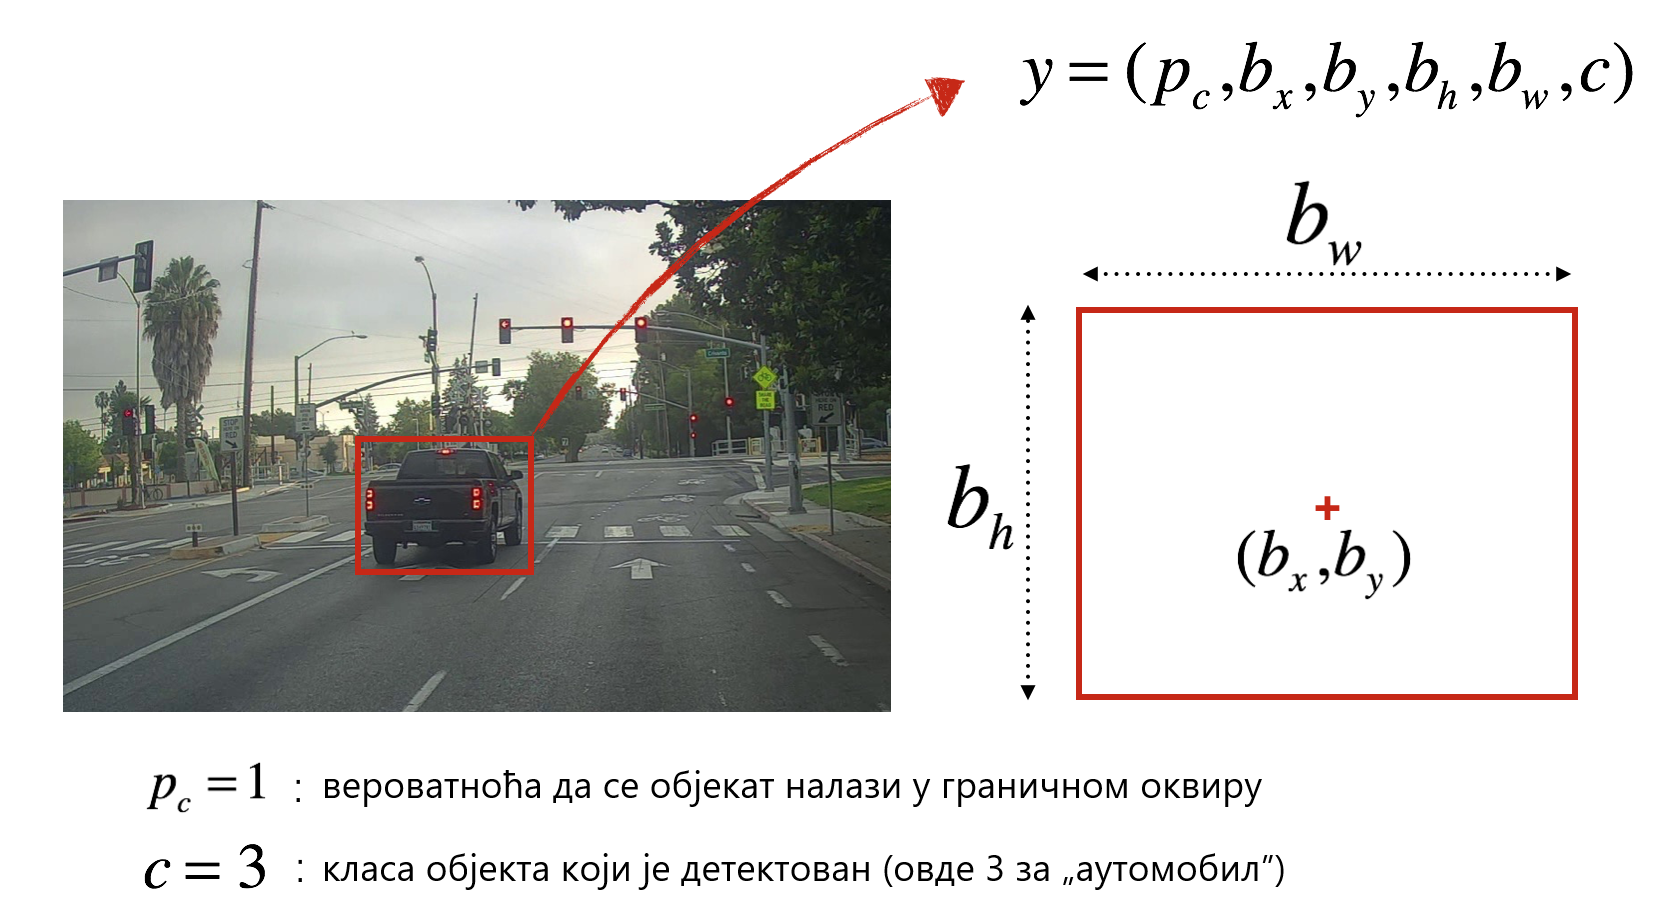
\includegraphics[scale=0.35]{slike/box_label.png}
  \caption{Детекција и дефинисање граничног оквира око објекта}
  \label{fig:bb_auto}
\end{figure}

Параметар $c$ може да буде или целобројна вредност која представља класу или
вектор димензија броја класа које детектујемо, где члан вектора који
представља класу има вредност $1$, а остали имају вредност нула.

Ако би требало да детектујемо три класе:
\begin{enumerate}
 \item пешак
 \item аутомобил
 \item мотоцикл
\end{enumerate}
вектор којим се представља детекција \textit{аутомобила}, где $c$ је
представљено као вектор тј.\ постоји посебан члан (бит) за
сваку класу, изгледао би као:
\begin{equation}
y =
\begin{bmatrix}
 p_c \\
 b_x \\
 b_y \\
 b_h \\
 b_w \\
 c_1 \\
 c_2 \\
 c_3
\end{bmatrix}
=
\begin{bmatrix}
 1 \\
 b_x \\
 b_y \\
 b_h \\
 b_w \\
 0 \\
 1 \\
 0
\end{bmatrix}
\label{eq:detResKl}
\end{equation}

У случају да у посматраној слици нема објеката, вероватноћа $p_c$ ће бити
0, па су остали чланови вектора небитни:
\begin{equation}
y =
\begin{bmatrix}
 p_c \\
 b_x \\
 b_y \\
 b_h \\
 b_w \\
 c_1 \\
 c_2 \\
 c_3
\end{bmatrix}
=
\begin{bmatrix}
 0 \\
 ? \\
 ? \\
 ? \\
 ? \\
 ? \\
 ? \\
 ?
\end{bmatrix}
\label{eq:detNoResKl}
\end{equation}

На слици \ref{fig:ng_slidW} је приказан пример
\textit{Детекције објеката клизним прозорима} \cite{ngObjDet}.
Сваки \textit{прозор} се проследи конволуцијској мрежи, која
даје резултат да ли има објекта у прослеђеном исечку слике
или не. \textit{Прозор} треба да „проклиза” кроз целу слику
и овај поступак се може поновити и са већим
\textit{прозором}.

Идеја је да ће се сигурно унутар неког \textit{прозора}
наћи објекат тј.\ да ће резултат прослеђивања исечка слике
конволуцијској мрежи бити 1.

\begin{figure}[H]
  \centering
      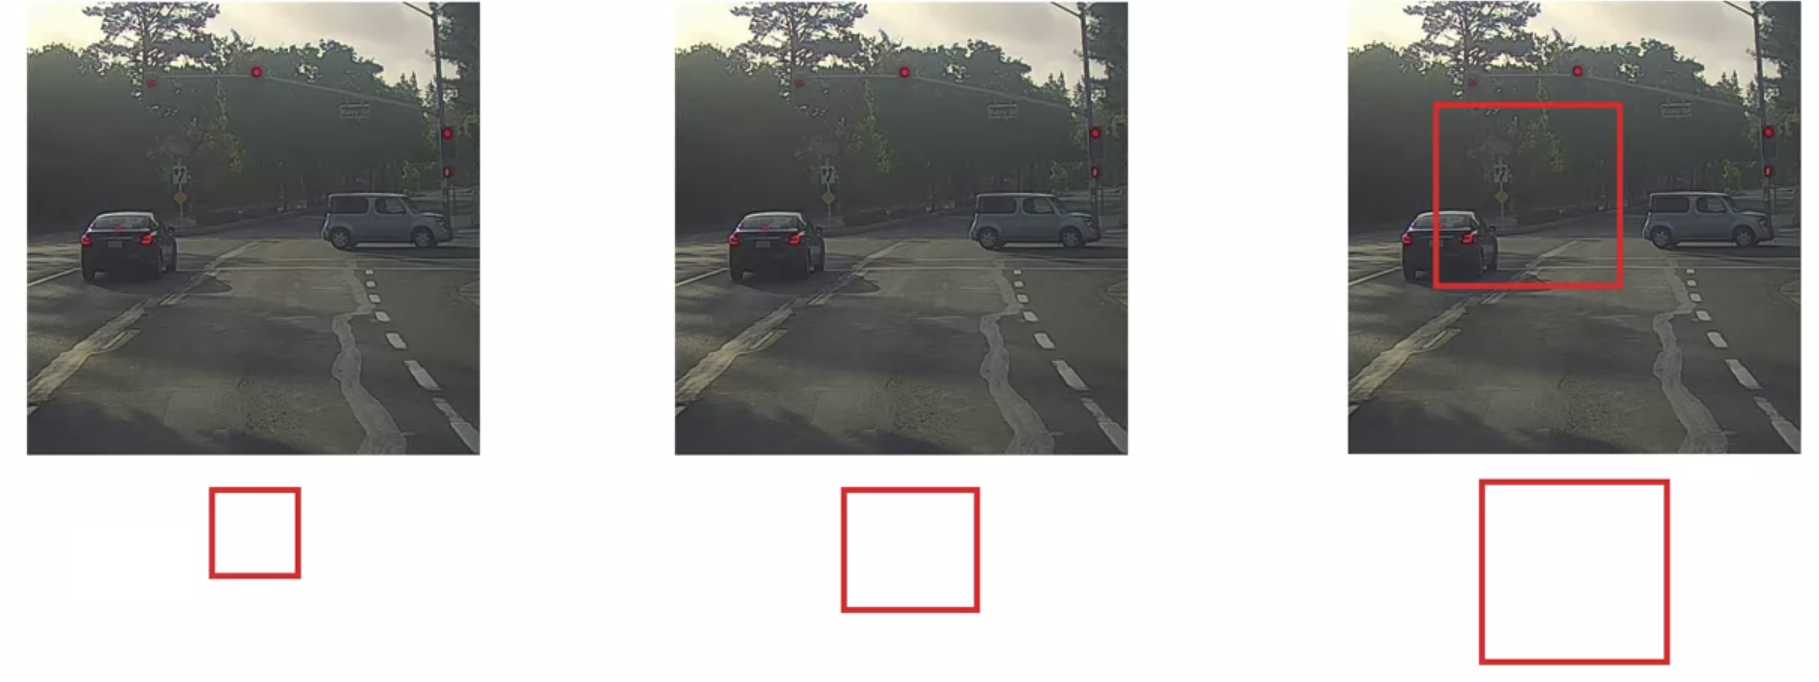
\includegraphics[scale=0.3]{slike/slidW.png}
  \caption{Детекција објеката клизним прозорима}
  \label{fig:ng_slidW}
\end{figure}

Проблем оваквог приступа је превелико време извршавања.
\textit{Детектор објеката клизним прозорима} се може
направити коришћењем конволуцијских мрежа и таква
имплементација је много ефикаснија.

Предност која се добија конволуцијском имплеметацијом је то што
је у једној итерацији могуће добити више вредности тј.\ резултата
за више \textit{прозора}. Слика \ref{fig:ng_slidWConv1} приказује
имплементацију \textit{детекције објеката клизним прозорима} применом
конволуцијских мрежа.

Прва мрежа на крају
садржи два \textit{потпуно повезана слоја} (\textit{fully connected layers}).
Ова два слоја праве проблем тј.\ успоравају детекцију, јер је
потребно посебно извршавање за сваки \textit{прозор} тј.\ исечак слике. На крају се
налази Softmax слој, чији сваки члан представља вероватноћу да је детектована класа
којој тај члан одговара.

У другом случају се примењује филтер \mbox{$5 \times 5 \times 16 \times 400$}, па
су излазне димензије \mbox{$1 \times 1 \times 400$}, а у наредном кораку се врши конволуција
коришћењем 400 филтера димензија $1 \times 1$. На крају се примењује $1 \times 1$ филтер чиме се добија
последњи слој димензија \mbox{$1 \times 1 \times 4$}.

\begin{figure}[H]
  \centering
      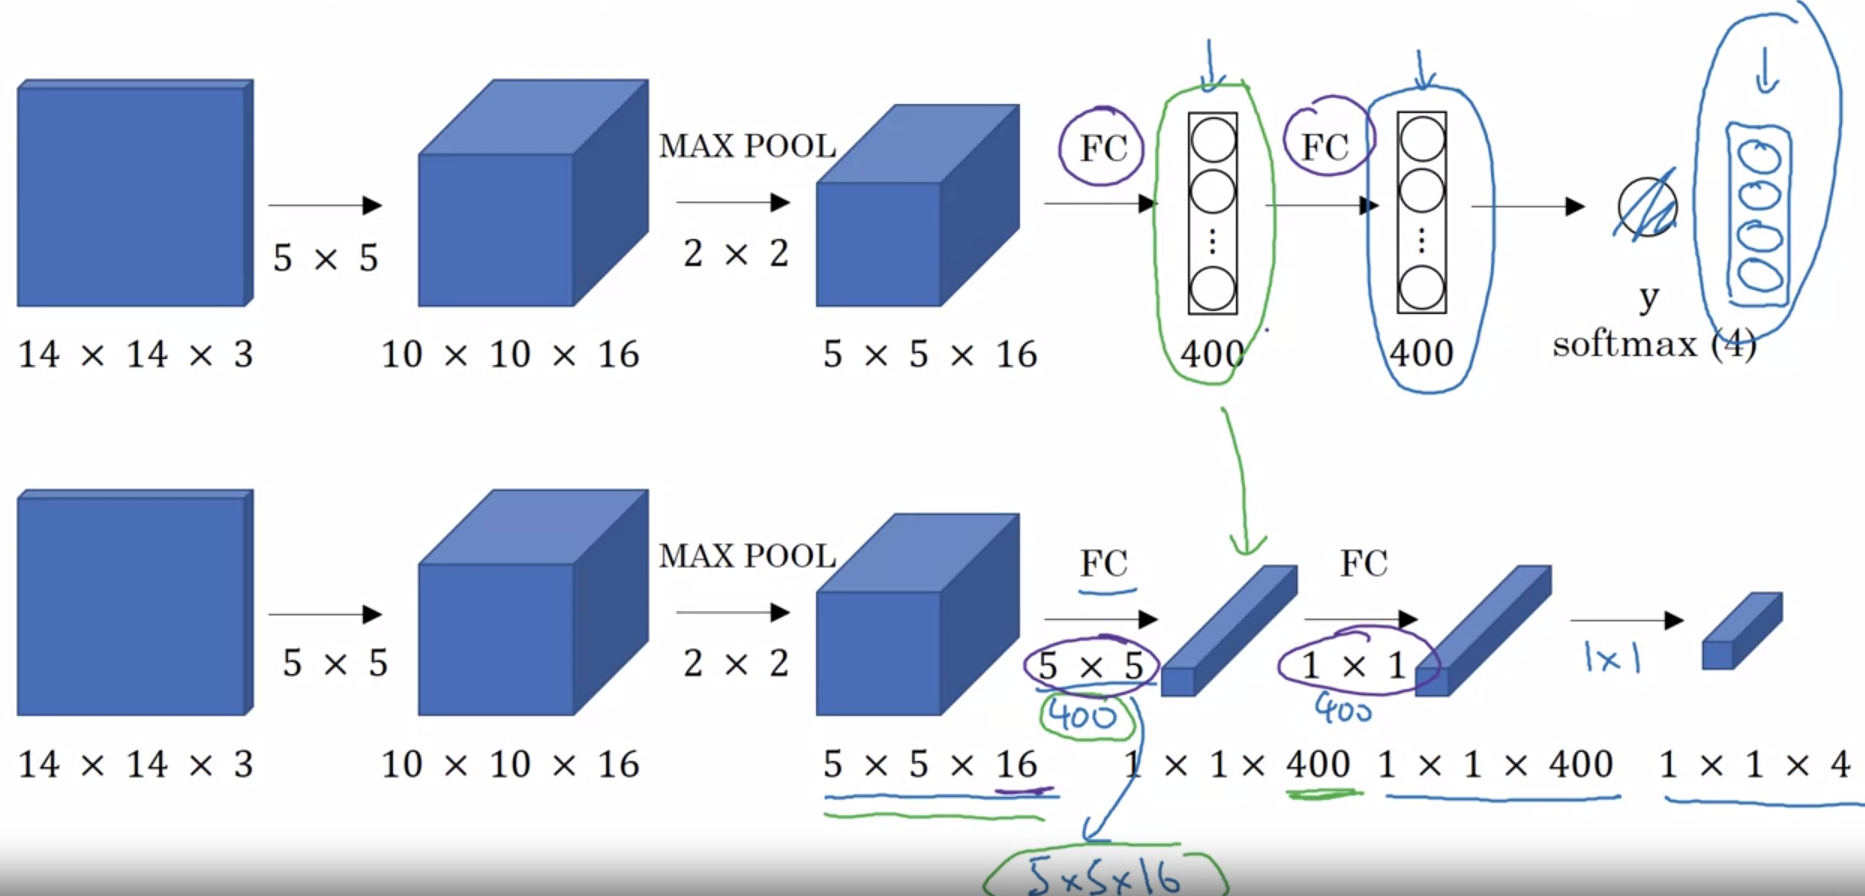
\includegraphics[scale=0.3]{slike/ngSlidWConv1.png}
  \caption{Имплементација клизних прозора применом конволуцијских мрежа}
  \label{fig:ng_slidWConv1}
\end{figure}

Слика \ref{fig:ng_slidWConv2} приказује случај када на улазу нађе слика
већих димензија од $14 \times 14$, као 	$16 \times 16$ или $28 \times 28$.

Сада се види предност у конволуцијској имплементацији
\textit{детекције објеката клизним прозорима}, где нпр.\ зелени
(\mbox{горњи-десни})
$14 \times 14$ исечак улазне слике, као резултат даје зелено означен
део излаза.
\newpage
Поента је да су једним извршавањем добијени разултати
за све исечке слике, исто је и за последњи пример када се на улазу нашла
слика димензија $28 \times 28$.

\begin{figure}[H]
  \centering
      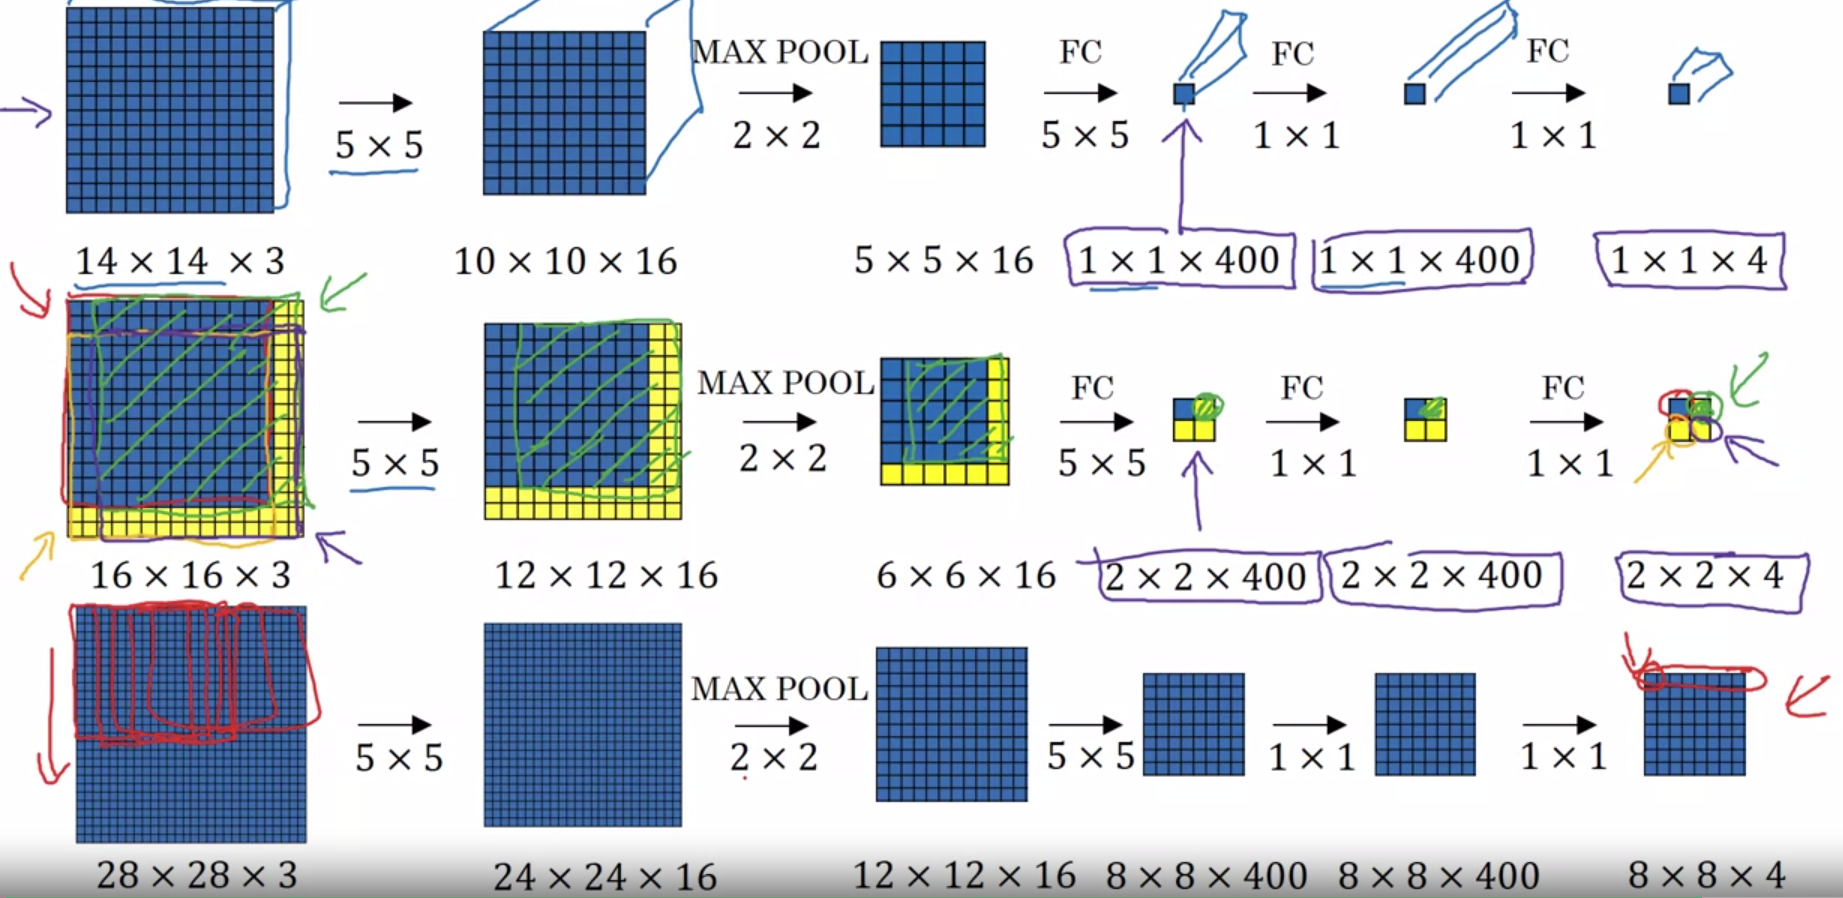
\includegraphics[scale=0.3]{slike/ngSlidWConv2.png}
  \caption{Детекција над сликама већих димензија}
  \label{fig:ng_slidWConv2}
\end{figure}

Наредна слика показује све позиције квадрата којим се праве исечци слике
унутар којих је потребно извршити детекцију. Као што је горе објашњено
вероватноће да се унутар квадрата налазе тражени објекти
(у овом случају аутомобил) се добијају истовремено за
све квадрате (исечке слике).

Конволуцијска имплементација је много ефикаснија него када се
посебно за сваки део слике врши тестирање.

\begin{figure}[H]
  \centering
      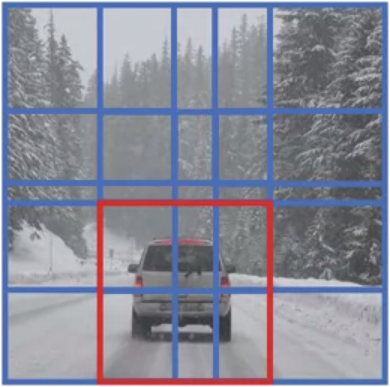
\includegraphics[scale=0.6]{slike/ngSlidWConv3.png}
  \caption{Истовремено извршавање детекција}
  \label{fig:ng_slidWConv3}
\end{figure}

Сада је потребно изабрати најбољи гранични оквир око објекта.
Оквир припада оном исечку слике у коме се налази центар оквира.
\newpage
Дефинисан је параметар
\textbf{ПпУ - Пресек преко Уније (IoU - Intersection over Union)},
којим је могуће установити преклапања два оквира.
Представља однос површина пресека два оквира и њихове уније.
\begin{equation}
IoU = \frac{\textcolor{yellow}{\cap}}{\textcolor{green}{\cup}}
\label{eq:ng_IoU}
\end{equation}

Слика \ref{fig:ng_IoU} приказује преклапање два оквира, где је
жутом бојом означен пресек, а зеленом унија, као
у једначини (\ref{eq:ng_IoU}).
Дефинише се и задовољавајући праг, па ако је $IoU \geq 0.5$ нађени
оквир се прихвата; наравно, овај праг је могуће повећати.
\begin{figure}[H]
  \centering
      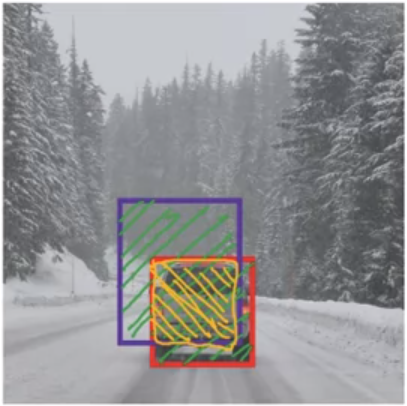
\includegraphics[scale=0.6]{slike/ngIoU.png}
  \caption{Преклапање два гранична оквира}
  \label{fig:ng_IoU}
\end{figure}

Слика \ref{fig:ng_NonMax1} приказује случај када се исти објекат
нађе унутар више граничних оквира, али такође сваки са различитом
сигурношћу указује да је тај објекат из одређене класе, у овом
случају су различите вероватноће да је нађен аутомобил.
\newpage
Узимају се у обзир оквири са највећом вероватноћом, а одбацују остали
оквири који имају велико преклапање тј.\ IoU дефинисан у
једначини (\ref{eq:ng_IoU}).

\begin{figure}[H]
  \centering
      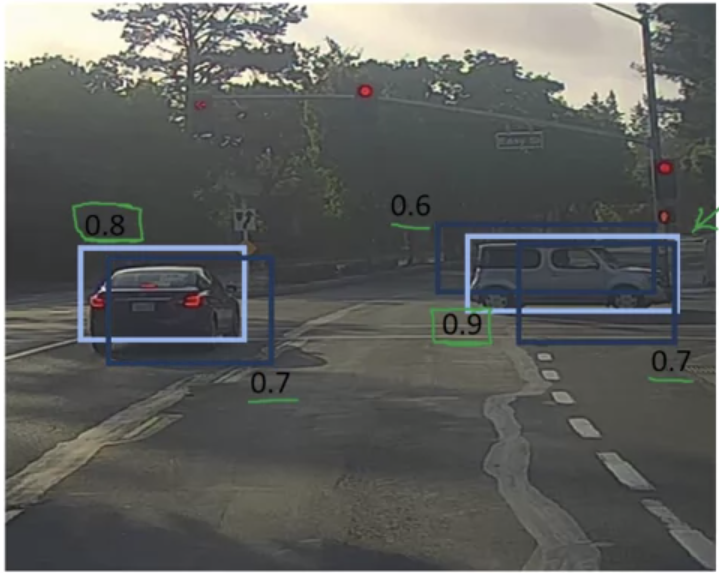
\includegraphics[scale=0.55]{slike/ngNonMax1.png}
  \caption{Више граничних оквира око истог објекта}
  \label{fig:ng_NonMax1}
\end{figure}

Овај поступак се назива \textbf{Не-Масимално потискивање (Non-Max suppression)}
и одбацују се тј.\ \textit{потискују} оквири који немају максималну вероватноћу
детекције.

Нека је сада резултат израчунавања тј.\ провере да ли се објекат налази
унутар прослеђеног исечка сличан као у приказаном вектору у
једначини (\ref{eq:detResKl}), али сада нека су изостављене класе, па
је претпоставка да се врши претрага само за аутомобил и излаз је:

\begin{equation}
y =
\begin{bmatrix}
 p_c \\
 b_x \\
 b_y \\
 b_h \\
 b_w
\end{bmatrix}
\label{eq:detRes}
\end{equation}

Поступак извршавања детекције је одеђен \mbox{псеудо-кодом}:
\begin{enumerate}[label=\arabic*)]
\item Одбацити све оквире где је вероватноћа $p_c \leq 0.6$
\item Док год има непроверених оквира:
  \begin{enumerate}[label=(\roman*)]
  \item Изабрати оквир са највећом вероватноћом $p_c$
  \item Одбацити све преостале оквире где је $IoU \geq 0.5$ у односу на
  оквир из претходног корака
  \end{enumerate}
\end{enumerate}
\newpage
Претрага се врши над сликом \ref{fig:ng_NonMax2}, која је подељена
\textit{решетком} димензија $19 \times 19$.

\begin{figure}[H]
  \centering
      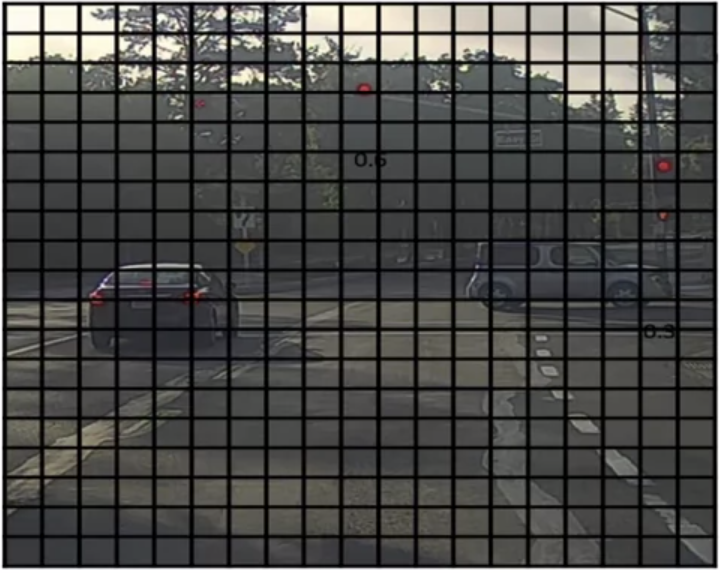
\includegraphics[scale=0.55]{slike/ngNonMax2.png}
  \caption{Слика подељена \textit{решетком} димензија $19 \times 19$}
  \label{fig:ng_NonMax2}
\end{figure}

Један од проблема детекције, који се може уочити до сада, је да се пољу
\textit{решетке} може доделити само један објекат \cite{ngAnchor}.
Слика \ref{fig:ng_Anchor1} приказује случај када центри граничних оквира
\textit{пешака} и \textit{аутомобила} припадају истом пољу.

\begin{figure}[H]
  \centering
      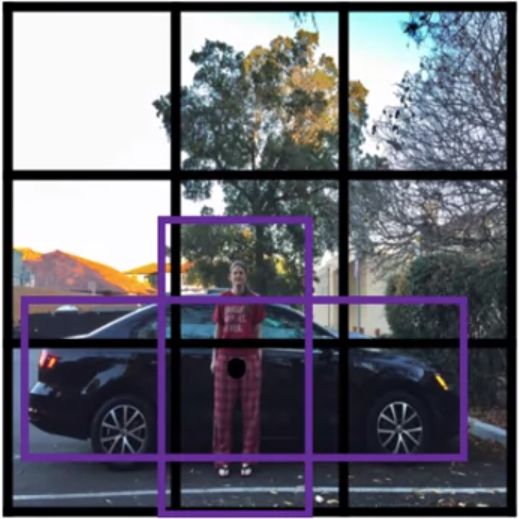
\includegraphics[scale=0.55]{slike/ngAnchor1.png}
  \caption{Класни оквири у случају више објеката додељеним једном пољу}
  \label{fig:ng_Anchor1}
\end{figure}

Овакав проблем се решава дефинисањем граничних оквира који
одговарају одређеној класи (\textbf{Anchor boxes}) и у овом случају постоје
два, један за \textit{пешака} и један за \textit{аутомобил}.

До сада смо сматрали да свако поље решетке као излаз даје вектор као у
једначини (\ref{eq:detResKl}) тј.\ до сада је резултат израчунавања био
$3 \times 3 \times 8$, где је сваком пољу био додељен вектор са 8 чланова
који дефинишу детекцију.

Сада је излаз $3 \times 3 \times 16$, а вектор је дуплиран и првих 8
чланова се односи на детекцију која одговара првом класном оквиру,
а других 8 другом.

\begin{equation}
y =
\begin{bmatrix}
 p_c \\
 b_x \\
 b_y \\
 b_h \\
 b_w \\
 c_1 \\
 c_2 \\
 c_3 \\
 \dots \\
 p_c \\
 b_x \\
 b_y \\
 b_h \\
 b_w \\
 c_1 \\
 c_2 \\
 c_3
\end{bmatrix}
=
\begin{bmatrix}
 1 \\
 b_x \\
 b_y \\
 b_h \\
 b_w \\
 1 \\
 0 \\
 0 \\
 \dots \\
 1 \\
 b_x \\
 b_y \\
 b_h \\
 b_w \\
 0 \\
 1 \\
 0
\end{bmatrix}
\label{eq:anchor1}
\end{equation}

Детектовани објекат се додељује пару
\verb (пољеРешетке,класниОквир)  \verb (gridCell,anchorBox) , а
објекат, са слике над којом се врши тренирање, се додељује оном
класном оквиру који има највеће преклапање са „правим” оквиром тј.\ највећи
IoU (једначина (\ref{eq:ng_IoU})).

Уколико се на слици налази само аутомобил, тада ће прва половина вектора, која
се односи на \textit{пешака}, имати исте вредности као и раније у
случају неналажења објекта,  као у једначини (\ref{eq:detNoResKl}).

Овако дефинисана примена класних оквира (Anchor boxes) не решава случај
када се у пољу \text{решетке} налазе три (или више) објеката, али с обзором
да YOLO алгоритам примењује \mbox{$19 \times 19$} \text{решетку} над сликом,
мале су шансе да ће се већи број објеката тј.\ центри граничних оквира
око њих наћи у истом пољу \text{решетке}.
Такође, могуће је да истом пољу припадају два објекта исте класе, па су
им и класни оквири (Anchor boxes) исти. Одређивање класних оквира
се може вршити произвољно (ручно) или применом K-means алгоритама, којим
се групишу слични објекти.

\newpage
\textbf{YOLO} (\textbf{You Only Look Once}) \textbf{алгоритам}
функционише применом наведених техника.
Нека се поново врши детекција \textit{пешака} и \textit{аутомобила};
а дефинисана су два класна оквира (Anchor boxes).
Уопштено, алгоритам функционише на следећи начин:
\begin{itemize}
 \item за сваку \textit{ћелију решетке} је потребно вратити 2 гранична
 оквира (слика \ref{fig:ng_YOLO12}, десно)
 \item занемарити оквире са малом вероватноћом детекције
 (слика \ref{fig:ng_YOLO34}, лево)
 \item за сваку класу је потребно извршити Не-Масимално
 потискивање (Non-Max suppression) (слика \ref{fig:ng_YOLO34}, десно)
\end{itemize}

\begin{figure}[H]
  \centering
      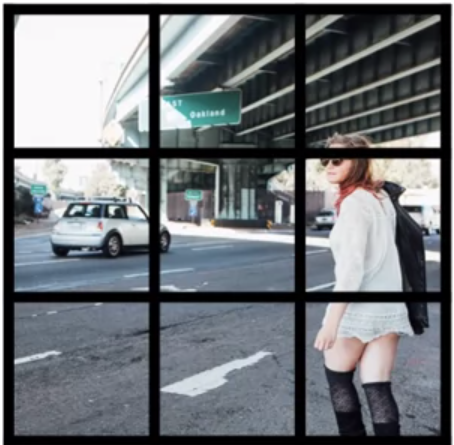
\includegraphics[scale=0.5]{slike/ngYOLO1.png}
      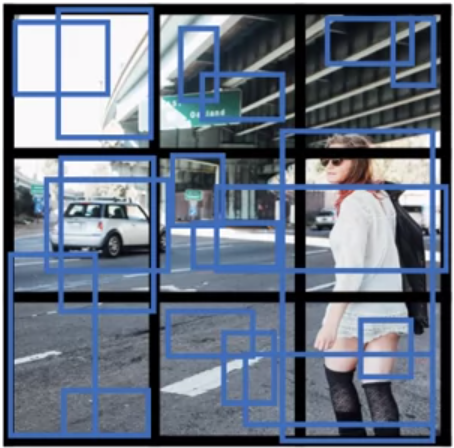
\includegraphics[scale=0.5]{slike/ngYOLO2.png}
  \caption{Тест слика; Оквири за сваку \textit{ћелију}}
  \label{fig:ng_YOLO12}
\end{figure}

\begin{figure}[H]
  \centering
      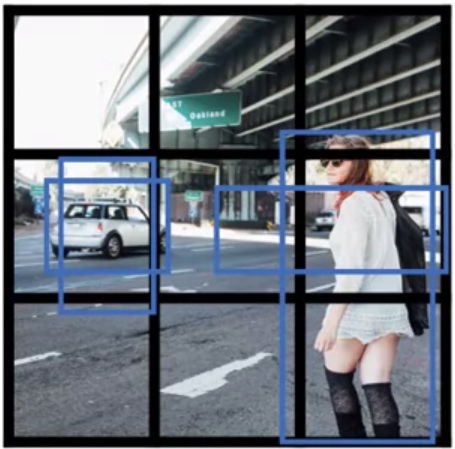
\includegraphics[scale=0.5]{slike/ngYOLO3.png}
      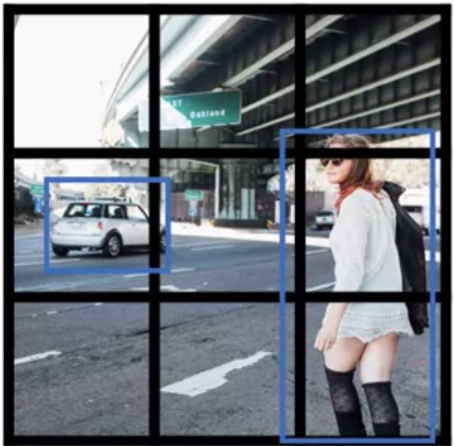
\includegraphics[scale=0.5]{slike/ngYOLO4.png}
  \caption{Оквири са великом вероватноћом поготка; Извршен Non-Max suppression}
  \label{fig:ng_YOLO34}
\end{figure}

Резултат алгоритма би требало да буде да су сви \textit{аутомобили} и
\textit{пешаци} на слици детектовани.

\newpage
\section{Тренирање - Darknet програмски оквир}
Darknet је програмски оквир за детекцију објеката у реалном времену и
представља имплементацију YOLO алгоритма. Написан је коришћењем
програмских језика C и CUDA, одакле и потиче изузетна брзина
овог система \cite{darknetSajt}.

Тренирање је извршено на GoogleColaboratory виртуелној машини.
Апликација се покреће тако што се \textit{Jupyter свеска},
која се налази на GoogleDrive налогу, отвори помоћу
GoogleColaboratory апликације.
Када се датотека отвори у претраживачу, апликација у позадини
алоцира ресурсе за виртуелну машину, после чега је могуће
извршавати \textit{ћелије} кода.
Jupyter свеска, коришћена уз апликацију GoogleColaboratory, наведена
је у литератури \cite{JupyterColab}.

После извршавања првих \textit{ћелија} где се клонира
GitHub репозиторијум Darknet-а, подешавају његови параметри,
извршава повезивање са GoogleDrive налогом,
потребно је валидациони и тренинг скуп пребацити у виртуелну
машину.

С обзиром да постоје 52 карте у шпилу тј.\ класе, параметре у
конфигурационој датотеци \verb yolov4-obj.cfg  треба прилагодити
тако да одговарају скупу који тренирамо.
Приказана су правила за дефинисање параметара:
\begin{itemize}
 \item \verb width  \verb =  \verb 416  и
 \verb height  \verb =  \verb 416 {} 
 
 (ова два параметра треба да буду дељиви са 32, 416
 је стандардна вредност, али се резултати могу побољшати са 608 и
 тренирање ће бити спорије)
 \item \verb max_batches  \verb =  \verb 104000 {}
 
 (\#класа) * 2000
 (не мање од 6000, па ако се тренира за 1, 2 или 3 класе биће 6000, али
 нпр.\ детектор са 5 класа има вредност \verb max_batches  \verb =  \verb 10000 )
 \item \verb steps=83200,93600 {} 
 
 (80\% \verb max_batches ),(90\% \verb max_batches )
 (у случају да је \verb max_batches  \verb =  \verb 10000 , онда је \verb steps  \verb =  \verb 8000,9000 )
 \item \verb filters  \verb =  \verb 171 {}
 \footnote{У датотеци је потребно
 пронаћи све параметре \textbf{classes} и поставити их на \textbf{52},
 а изнад сваког се налази конволуцијски слој који садржи параметар
 filters који треба изменити.}
 
 (\#класа + 5) * 3 (ако се врши тренирање
 за само једну класу, онда је \verb filters  \verb =  \verb 18 , али ако се тренира за 4
 класе онда \verb filters  \verb =  \verb 27 )
\end{itemize}

Датотека \verb cards.names  садржи називе класа (карата),
а датотека \verb cards.data  садржи више информација
(број класа; путању до датотеке са путањама до тренинг слика;
путању до датотеке која садржи путање до валидационих слика; путању до датотеке са називима класа;
директорујум где се чувају параметри истрениране мреже):
\begin{verbatim}
classes = 52
train = data/train.txt
valid = data/val.txt
names = data/cards.names
backup = /mydrive/Dokumenti/Fax/DiplomskiKarte/yolov4/backup
\end{verbatim}

Тренирање почиње од иницијалних вредности тежина веза
сачуваних у датотеци \verb yolov4.conv.137  и покреће се
командом:
\begin{minted}{python}
 ./darknet detector train data/obj.data cfg/yolov4-obj.cfg
			yolov4.conv.137 -dont_show -map
\end{minted}

Пре тестирања на слици или видеу, потребно је изменити
конфигурациону датотеку \verb yolov4-obj.cfg  и поставити
\verb batch=1  и \verb subdivisions=1 .

Тестирања над сликом и видеом се позивају следећим командама, респективно:
\begin{minted}{python}
./darknet detector test data/obj.data cfg/yolov4-obj.cfg
		/mydrive/yolov4/backup/yolov4-obj_last.weights
		/mydrive/images/car2.jpg -thresh 0.3
		
./darknet detector demo data/cards.data cfg/yolov4-obj.cfg
		/mydrive/Dokumenti/Fax/DiplomskiKarte/yolov4/
		      backup/yolov4-obj_last.weights
		-dont_show /mydrive/Dokumenti/Fax/DiplomskiKarte/
			  video/videoTep.mp4
		-thresh 0.8 -i 0 -out_filename /mydrive/Dokumenti
		    /Fax/DiplomskiKarte/video/videoTep_08Thresh.avi
\end{minted}

Параметар \verb -thresh  \verb 0.8  омогућава да се као
резултат прикажу само оне детекције где је верoватноћа $\geq 0.8$.

\begin{figure}[H]
  \centering
      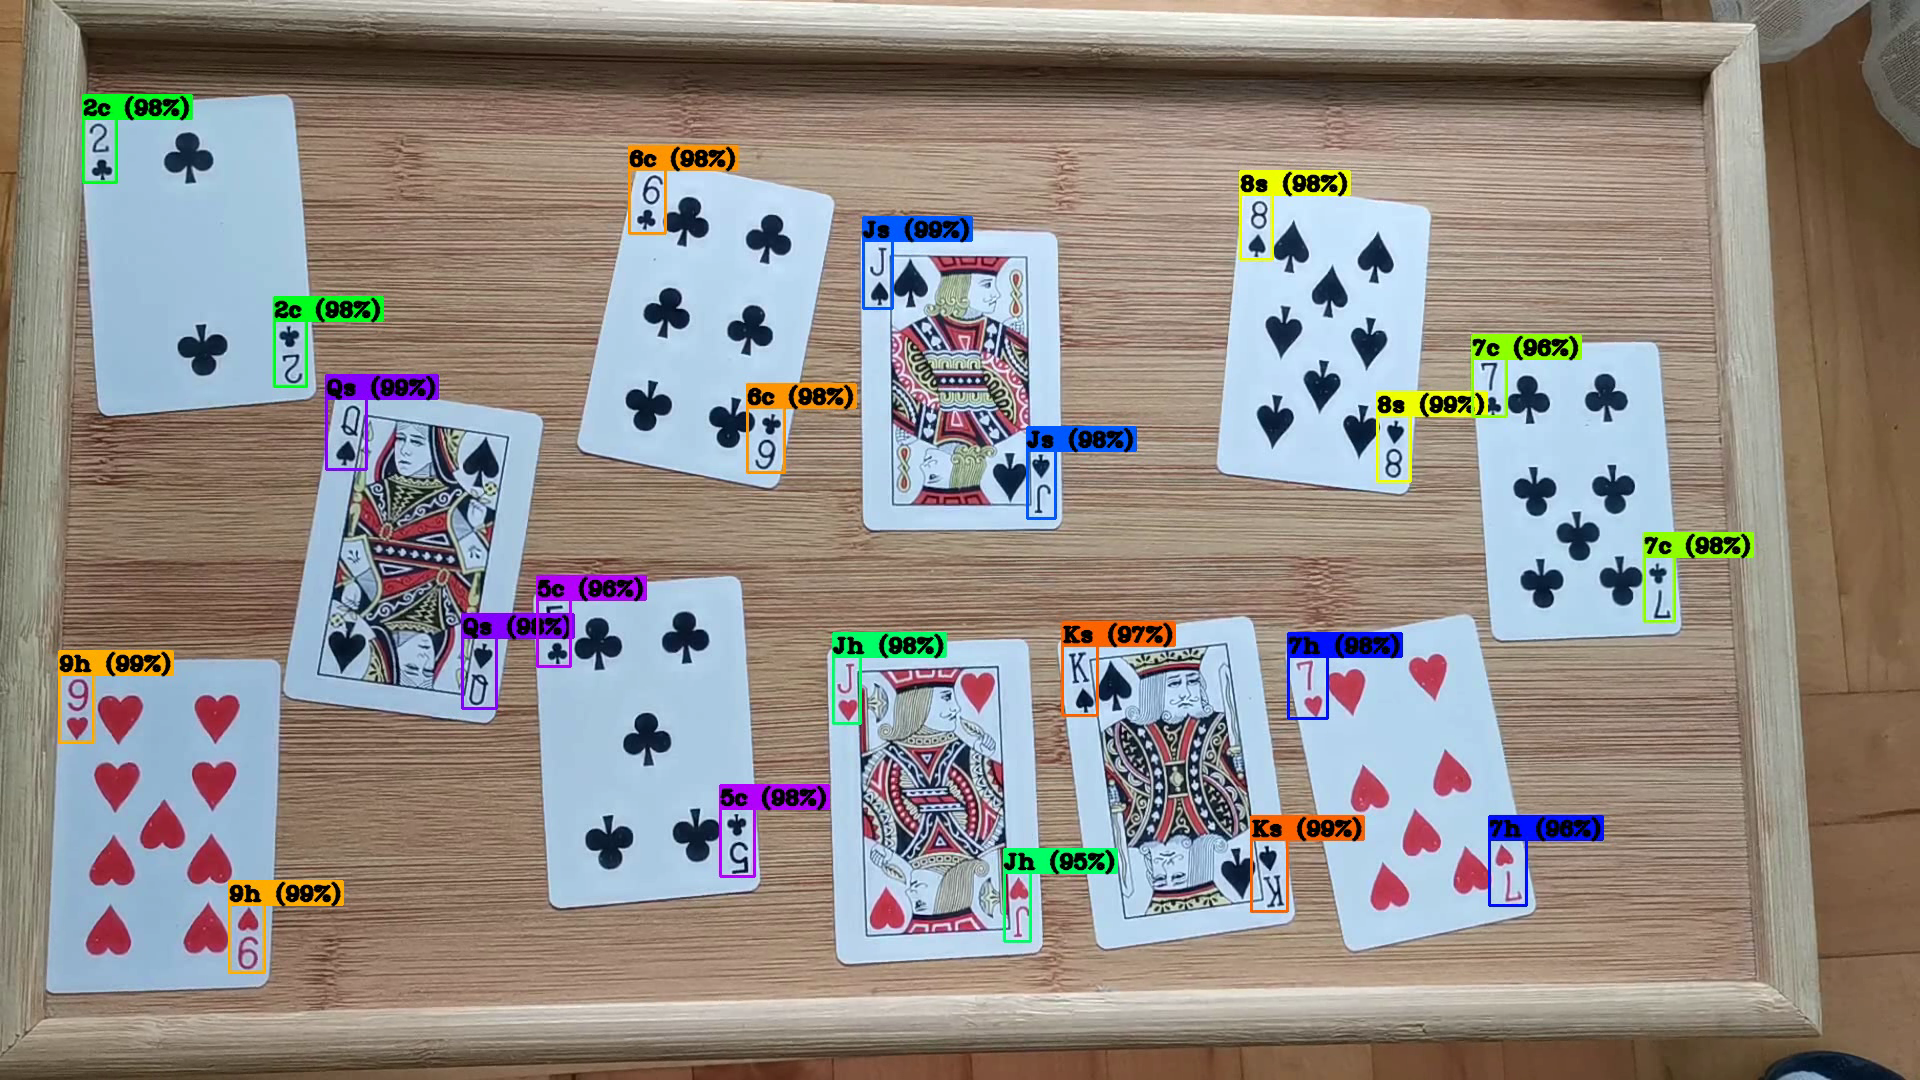
\includegraphics[scale=0.29]{slike/TestVideo.png}
  \caption{Тестирање над видеом}
  \label{fig:TestVideo}
\end{figure}

Детекција у релном времену са WEB камере се покреће
командом:
\begin{minted}{python}
./darknet detector demo data/cards.data cfg/yolov4-obj.cfg
		/mydrive/Dokumenti/Fax/DiplomskiKarte/yolov4/
		      backup/yolov4-obj_last.weights -c 0
\end{minted}

\subsection{Промене конфигурација током тренирања}
Направљен је тренинг скуп који садржи 50000 слика и
валидациони од 10000 (20\% тренинг скупа).

Тренирање мреже је покренуто са изнад наведеним параметрима,
али с обзиром да је \textit{дужинa корака при учењу}
(\textit{lerning rate}) била превелика, за финије
подешавање је било потребно поставити овај параметар на
вредност 0.0001 \cite{YTkarte}.
Тренирање са мањом вредношћу параметра \mbox{\textit{lerning rate}}
је покренуто од 3000.\ итерације и већ на 3400.\ итерацији
резултати при тестирању су били врло добри.

На 3000.\ итерацији мера тачности мреже над тренинг скупом
(Mean Average Precission - mAP) је била око 97.5\% и
при тестирању над видеом детекције нису биле тачне.

После тренирања од још 400 итерација
са мањом вредношћу параметра \mbox{\textit{lerning rate}},
Mean Average Precission - mAP је износио 100\% над тренинг скупом.
Команда за израчунавање mAP:
\begin{minted}{python}
./darknet detector map data/cards.data cfg/yolov4-obj.cfg 
      /mydrive/Dokumenti/Fax/DiplomskiKarte/yolov4/
		    backup/yolov4-obj_3400.weights
\end{minted}


Извршене су измене параметара \verb width  и \verb height  и
постављени на 608, да би мрежа била боље прилагођена
већој резолуцији камере.

На крају су коришћени тежински коефицијенти
после извршених 5400 итерацијa.

\subsection{Резултати тренирања}

У GitHub репозиторијуму \textit{Diplomski rad - YOLO detekcija},
наведеном у литератури \cite{git_moj}, се налазе:
\begin{itemize}
 \item тежински коефицијенти истрениране мреже
 \item снимак над којим је извршена детекција
 \item пример снимка карте под различитим осветљењем,
  који је коришћен за прављење слика тренинг скупа
 \item \LaTeX{} код овог рада
\end{itemize}



\newpage
\section{Закључак}
Један од изазова оваквог пројекта је
то што је програм потребно прилагодити стварним (физичким)
објектима. При припреми тренинг скупа треба снимити
карте под што разноврснијим осветљењем, шпил карата мора
да буде прецизно одштампан, подлога на којој се налази карта
треба да буде неутрална \dots 

Конфигурационе параметре тренирања над скупом је потребно
мењати у складу са побољшањем, у виду смањивања
функције трошка и повећања тачности над тренинг скупом.
С обзиром да тренирање траје неколико сати, резултат
промене неких параметара није одмах видљив и
узима много времена.

Теоријиски део у раду je наведен да би се стекао увид
у начин рада алгоритма.
\mbox{YOLO (You Only Look Once) алгоритам} је невероватно ефикасан, а то све
због приступа да се слика посматра као целина и у једној итерацији
извршава детекција (не извршавају се детекције над деловима слике, а
у наредној итерацији збирно посматрају резултати, ово је спорије и
тај приступ имају неки други алгоритми).

YOLO алгоритам за детекцију у реалном времену је изузетно моћан
и може бити примењен над произвољним објектима.
Треба имати у виду да може бити примењен и
за посматрања на јавним местима. Главни
аутор рада o YOLO алгоритму, Joseph Redmon, је радио
и на развоју имплементације алгоритма,
Darknet програмском оквиру, и повукао се са пројекта из
етичких разлога, јер је био забринут за угрожавање
приватности људи, а
алгоритам је био употребљаван и у војне сврхе.

Задивљујућа је чињеница да је сада рачунар способан да \textit{види},
а да су теоријске идеје изнете у овом раду 
и библиотеке заступљене у области Машинског учења
први пут имплементиране
у блиској прошлости.

Несумњиво је да ће, по речима мог ментора,
\textit{развој Вештачке интелигенције обележити наше каријере}.

%\newpage
\clearpage
\begingroup
\raggedright
%\bibliography{srpski_Literatura}


\begin{thebibliography}{99}

\bibitem{git_karte}
\textit{playing-card-detection}, приступљено (септембар 2020.) на
\url{https://github.com/geaxgx/playing-card-detection.git}

\bibitem{stack_slika}
api55. Одговор на: \textit{What's the theory behind computing variance of an image?}
[Интернет форум]. Приступљено (септембар 2020.) на
\url{https://stackoverflow.com/questions/48319918/whats-the-theory-behind-computing-variance-of-an-image}

\bibitem{cv2_kontura}
\textit{Contours : Getting Started}, приступљено (септембар 2020.) на
\url{https://docs.opencv.org/trunk/d4/d73/tutorial_py_contours_begin.html}

\bibitem{cv2_piksel}
\textit{Morphological Transformations}, приступљено (септембар 2020.) на
\url{https://opencv-python-tutroals.readthedocs.io/en/latest/py_tutorials/py_imgproc/py_morphological_ops/py_morphological_ops.html}

\bibitem{py_pickle}
\textit{pickle — Python object serialization}, приступљено (септембар 2020.) на
\url{https://docs.python.org/3/library/pickle.html}

\bibitem{git_YOLOformat}
AlexeyAB. Одговор на: \textit{Specific format of annotation}
[Интернет форум]. Приступљено (септембар 2020.) на
\url{https://github.com/AlexeyAB/Yolo_mark/issues/60}

\bibitem{nn_osnova}
\textit{Machine Learning for Beginners: An Introduction to Neural Networks}, приступљено (септембар 2020.) на
\url{https://towardsdatascience.com/machine-learning-for-beginners-an-introduction-to-neural-networks-d49f22d238f9}

\bibitem{stackex_loss}
lejlot. Одговор на: \textit{Objective function, cost function, loss function: are they the same thing?}
[Интернет форум]. Приступљено (септембар 2020.) на
\url{https://stats.stackexchange.com/questions/179026/objective-function-cost-function-loss-function-are-they-the-same-thing}
%%%%%%%%%%%%%%%%%%%%%%%%%%
\bibitem{ngCVision}
Andrew Ng, \textit{Computer Vision}, [Интернет курс] \textit{Convolutional
Neural Networks}, приступљено (септембар 2020.) на
\url{https://www.coursera.org/learn/convolutional-neural-networks/lecture/Ob1nR/computer-visions}

\bibitem{ngEdgeDet}
Andrew Ng, \textit{Edge Detection Example}, [Интернет курс] \textit{Convolutional
Neural Networks}, приступљено (септембар 2020.) на
\url{https://www.coursera.org/learn/convolutional-neural-networks/lecture/4Trod/edge-detection-example}

\bibitem{ngMoreEdge}
Andrew Ng, \textit{More Edge Detection}, [Интернет курс] \textit{Convolutional
Neural Networks}, приступљено (септембар 2020.) на
\url{https://www.coursera.org/learn/convolutional-neural-networks/lecture/8Donz/more-edge-detection}

\bibitem{ngConvOneLay}
Andrew Ng, \textit{One Layer of a Convolutional Network}, [Интернет курс] \textit{Convolutional
Neural Networks}, приступљено (септембар 2020.) на
\url{https://www.coursera.org/learn/convolutional-neural-networks/lecture/nsiuW/one-layer-of-a-convolutional-network}
%%%%%%%%%%%%%%%%%%%%%%%%%%
\bibitem{ngObjLoc}
Andrew Ng, \textit{Object Localization}, [Интернет курс] \textit{Convolutional
Neural Networks}, приступљено (септембар 2020.) на
\url{https://www.coursera.org/learn/convolutional-neural-networks/lecture/nEeJM/object-localization}

\bibitem{ngObjDet}
Andrew Ng, \textit{Object detection}, [Интернет курс] \textit{Convolutional
Neural Networks}, приступљено (септембар 2020.) на
\url{https://www.coursera.org/learn/convolutional-neural-networks/lecture/VgyWR/object-detection}

\bibitem{ngSlidWConv}
Andrew Ng, \textit{Convolutional Implementation of Sliding Windows}, [Интернет курс] \textit{Convolutional
Neural Networks}, приступљено (септембар 2020.) на
\url{https://www.coursera.org/learn/convolutional-neural-networks/lecture/6UnU4/convolutional-implementation-of-sliding-windows}

\bibitem{ngAnchor}
Andrew Ng, \textit{Convolutional Implementation of Sliding Windows}, [Интернет курс] \textit{Convolutional
Neural Networks}, приступљено (септембар 2020.) на
\url{https://www.coursera.org/learn/convolutional-neural-networks/lecture/yNwO0/anchor-boxes}

\bibitem{darknetSajt}
\textit{Darknet: Open Source Neural Networks in C}, приступљено (септембар 2020.) на
\url{https://pjreddie.com/darknet/}

\bibitem{JupyterColab}
\textit{Running a YOLOv4 Object Detector with Darknet in the Cloud! (GPU ENABLED)}, приступљено (септембар 2020.) на
\url{https://colab.research.google.com/drive/1_GdoqCJWXsChrOiY8sZMr_zbr_fH-0Fg?usp=sharing}

\bibitem{YTkarte}
\textit{Playing card detection with YOLO}, приступљено (септембар 2020.) на
\url{https://youtu.be/pnntrewH0xg}

\bibitem{git_moj}
\textit{Diplomski rad - YOLO detekcija}, приступљено (септембар 2020.) на
\url{https://github.com/aleksavelickovic5762015/Diplomski-rad---YOLO-detekcija.git}

\end{thebibliography}

\endgroup

\end{document}